\documentclass[12pt]{article}
\usepackage[a4paper, total={7in,10in}]{geometry}

\usepackage{polyglossia}
\usepackage{ragged2e}
\usepackage{amsmath}
\usepackage{amssymb}
\usepackage{microtype}
\usepackage{graphicx}
\usepackage{changepage}
\usepackage{hyperref}
\usepackage{cancel}
\usepackage{wrapfig}
\usepackage{needspace}
\usepackage{mathtools}
\usepackage{caption}



\let\ORIincludegraphics\includegraphics
\renewcommand{\includegraphics}[2][]{\ORIincludegraphics[scale=0.65,#1]{#2}}
\newcommand{\verteq}{\rotatebox{90}{$\,=$}}
\newcommand{\equalto}[2]{\underset{\scriptstyle\overset{\mkern4mu\verteq}{#2}}{#1}}
\let\oldint\int
\let\oldiint\iint
\let\oldoint\oint
\let\oldsum\sum
\let\oldlim\lim
\renewcommand{\int}{\oldint\limits}
\renewcommand{\oint}{\oldoint\limits}
\renewcommand{\iint}{\oldiint\limits}
\renewcommand{\sum}{\oldsum\limits}
\renewcommand{\lim}{\oldlim\limits}

\graphicspath{{./images/}}
\setmainlanguage{russian}
\setotherlanguage{english}
\newfontfamily\russianfont[Script=Cyrillic]{Times New Roman}
\newfontfamily\englishfont{Times New Roman}
\setlength{\parindent}{0em}
\setlength{\parskip}{6pt}

\def\posl#1#2{\{#1_{#2}\}}
\DeclareMathOperator*{\sh-like}{\sinh-like}
\DeclareMathOperator*{\ch-like}{\cosh-like}
\DeclareMathOperator*{\th-like}{\tanh-like}
\DeclareMathOperator*{\cth-like}{\coth-like}
\DeclareMathOperator*{\tg-like}{\tan-like}
\DeclareMathOperator*{\ctg-like}{\cot-like}
\DeclareMathOperator*{\arctg-like}{\arctan-like}
\DeclareMathOperator*{\arcctg-like}{\arctan-like}

\setcounter{section}{7}

\begin{document}
    \justifying
    \begin{titlepage}
        \begin{center}
            \begin{center}
              
\includegraphics[scale=0.1]{logo.jpg}
            \end{center}
            \normalsize{МИНИСТЕРСТВО НАУКИ И ВЫСШЕГО ОБРАЗОВАНИЯ РОССИЙСКОЙ ФЕДЕРАЦИИ}\\
            \footnotesize{ФЕДЕРАЛЬНОЕ ГОСУДАРСТВЕННОЕ АВТОНОМНОЕ ОБРАЗОВАТЕЛЬНОЕ УЧРЕЖДЕНИЕ}\\ 
            \footnotesize{ВЫСШЕГО ОБРАЗОВАНИЯ}\\
            \small{\textbf{«Дальневосточный федеральный университет»}}\\
            \noindent\rule{17cm}{0.4pt}\\
            \large{\textbf{ИНСТИТУТ МАТЕМАТИКИ И КОМПЬЮТЕРНЫХ ТЕХНОЛОГИЙ}}\\
             \hfill \break
            \large{\textbf{Департамент программной инженерии и искусственного интеллекта}}\\
            \hfill\break
            \hfill \break
            \hfill \break
            \hfill \break
            \large{\textbf{ЛЕКЦИОННЫЙ МАТЕРИАЛ}}\\
            \begin{center}
              \normalsize{по дисциплине "Математический Анализ"}\\
              \normalsize{по образовательной программе подготовки бакалавров по направлению}\\
              \normalsize{02.03.03тп - Математическое Обеспечение и Администрирование Информационных систем}\\
              \normalsize{семестры обучения III-IV}
            \end{center}
            \hfill \break
            \hfill \break
            \hfill \break
            \begin{flushright}
                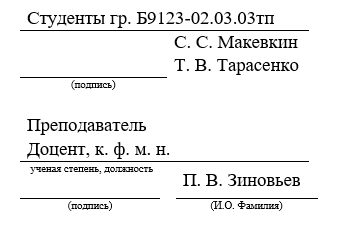
\includegraphics[scale=1.5]{rospis.png}
            \end{flushright}
            \hfill \break
            
            \end{center}
            \hfill \break
            \normalsize{ 
            
            }
            \begin{center} Владивосток \\ 2025 \end{center}
            \thispagestyle{empty}
    \end{titlepage}
    \pagebreak
    \tableofcontents
    \pagebreak
  \section{Криволинейные, кратные и поверхностные интегралы}
  \subsection{Криволинейные интегралы I рода}
  \underline{Определение: } Кривая $\overline{r}(t)=x(t)\overline{i}+y(t)\overline{j}$
  $a \leq t \leq b$ называется непрерывной гладкой кривой, если x(t),y(t),z(t) непрерывно дифференцируемы
  на [a;b] и $x'(t)^2+y'(t)^2+z'(t)^2 \not = 0$\\
  \underline{Определение: } Кривая называется непрерывной кусочно-гладкой кривой, если она состроит из конечного числа
  гладких кривых.\\
  Рассмотрим непрерывную кусочно-гладкую кривую:\\
  \begin{minipage}{0.45\textwidth} % Левая колонка — для изображения
      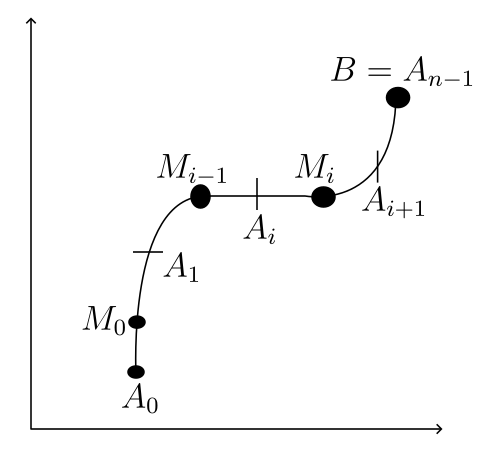
\includegraphics[width=\linewidth]{8.1.1.png}
  \end{minipage}%
  \hspace{1em} % Горизонтальный отступ между колонками
  \begin{minipage}{0.65\textwidth} % Правая колонка — для текста
      Пусть кривая имеет массу $\rho=\frac{\mathrm{kg}}{\mathrm{m}}$.
      \begin{enumerate}
        \item R
        \item В каждой элементарной $\Delta l_i$ выберем\\ произвольную $M_i$ 
        \item Вычислим $\rho(M_i)$
        \item Считаем, что на всём $\Delta l_i \rho=const=\rho(M_i)$
        \item Составим $\sigma_R=\sum_{i=0}^{n-1}\rho(M_i)\Delta l_i$
        \item $\lim_{\lambda_R \to 0} \sigma_R = m = \int_{(l)} g dl$
      \end{enumerate}
  \end{minipage}
  \vspace{1em}
  \par Рассмотрим функцию Z=f(x,y), заданную вдоль непрерывной кусочно-гладкой кривой l\\

  \begin{minipage}{0.45\textwidth}
    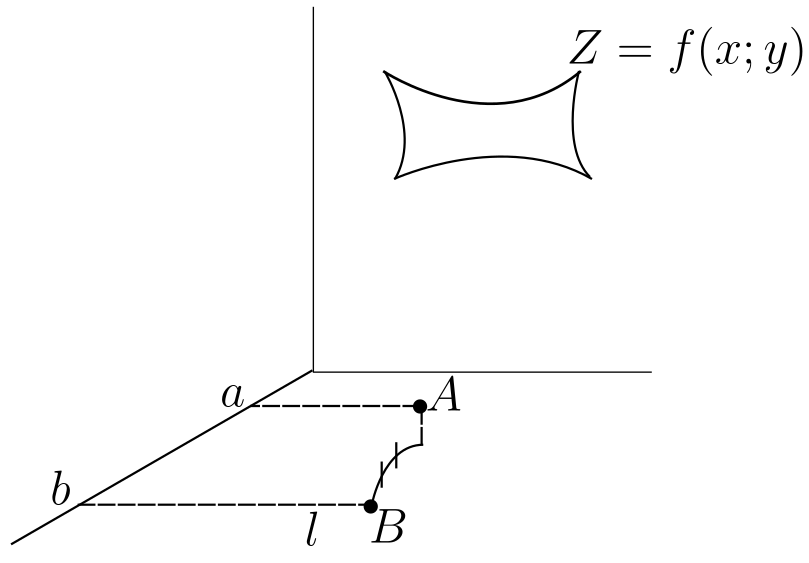
\includegraphics[scale=0.6]{8.1.2.png}
  \end{minipage}
  \hspace{1em} % Горизонтальный отступ между колонками
  \begin{minipage}{0.65\textwidth} % Правая колонка — для текста
      Пусть кривая имеет массу $\rho=\frac{\mathrm{kg}}{\mathrm{m}}$.
      \begin{enumerate}
        \item R
        \item Выберем произвольную (.) $M_i \in \Delta l_i$\\ (.)$M_i (\xi_i;\eta_i)$
        \item Вычислим $f(\xi_i;\eta_i)$
        \item Составим $\sigma_R = \sum_{i=0}^{n-1} f(\xi_i,\eta_i) \Delta l_i$
        \item Вычислим $\lim_{\lambda_R \to 0} \sigma_R = \int_{(l)} f(x;y) dl$
      \end{enumerate}
  \end{minipage}
  \vspace{1em}
  \par
  \underline{Определение: } Если существует конечный предел интегральной суммы $\sigma_R$, не 
  зависящей от способа разбиения кривой и выбора $(.) M_i(\xi_i,\eta_i)$, то он называется
  криволинейным интегралом I рода от функции f(x;y) по кривой l.\\
  \[m=\int_{(l)} f(x;y) dl\]\\
  \underline{Замечание:} Если кривая (AB) не замкнута: \[\int_{(AB)} f(x;y)dl = \int_{(BA)} f(x;y)dl\]
  !!! При переходе к определенному интегралу пределы интегрирования ставятся по мере возрастания
  переменной интегрирования.

  \begin{minipage}{0.45\textwidth}
    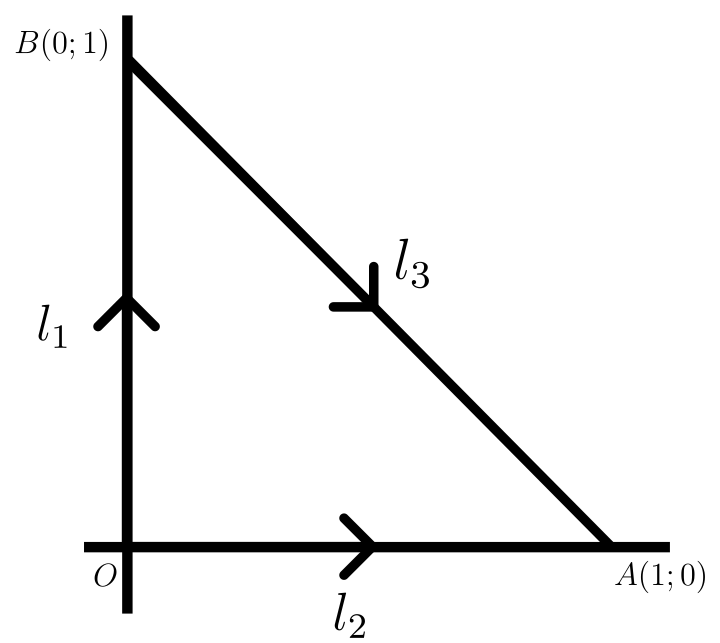
\includegraphics[scale=0.6]{8.1.3.png}
  \end{minipage}
  \hspace{1em}
  \begin{minipage}{0.65\textwidth}
      \[\int = \int_{(l_1)}+\int_{(l_2)}+\int_{(l_3)}\]\\
      \[\int_{0}^{1}\dots dy+\int_{0}^{1}\dots dx+\int_{0}^{1}\dots dx\]
  \end{minipage}
  \vspace{1em}
  \par
  \underline{Замечание:} Аналогично вводится интеграл по пространственной кривой $\int_{(l)} f(x;y;z)dl$
  \subsection{Вычисление криволинейного интеграла I рода.}
  \[\int_{(l)} f(x;y) dl \hspace{10pt} l: \begin{cases}
    x=x(t) & a\leq t\leq b\\
    y=y(t)
  \end{cases}\] \\
  \begin{minipage}{0.45\textwidth}
    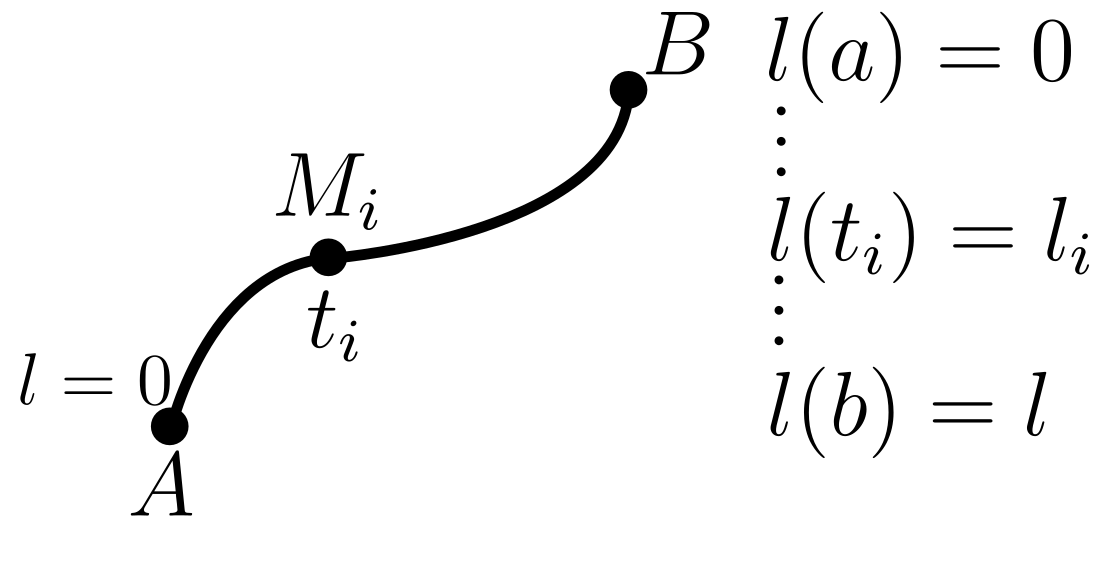
\includegraphics[scale=0.4]{8.2.1.png}
  \end{minipage}
  \hspace{1em}
  \begin{minipage}{0.65\textwidth}
    Положение (.) $M_i$ однозначно определяется с помощью \\
    длины дуги, отсчитываемой от (.)A. $\begin{cases}
      x=x(l)\\
      y=y(l)
    \end{cases}$
  \end{minipage}
  \vspace{1em}
  \par
  \[\int_{(l)}f(x;y)dl=\int_{0}^{l} f(x(l);y(l))dl\]
  \begin{enumerate}
    \item Если кривая задана уравнением y=f(x) $a \leq x \leq b$\\
    \[\int_{(l)} g(x;y)dl = \int_{a}^{b} f(x) \underbrace{\sqrt{1+f'(x)^2}dx}_{dl}\]
    \item Если кривая задана параметрически\\
    \[\begin{cases}
      x=x(t)\\
      y=y(t)
    \end{cases} t_1 \leq t \leq t_2 \hspace{20pt} \int_{(l)}g(x;y)dl=\int_{t_1}^{t_2}g(x(t);y(t))
    \sqrt{x'(t)^2+y'(t)^2}dt\]
    \item Если кривая задана $r=r(\phi) \hspace{20pt} \alpha \leq \varphi \leq \beta$\\
    \[\int_{(l)}g(x;y)dl = \int_{\alpha}^{\beta} g(r(\varphi)\cos(\varphi);r(\varphi)\sin(\varphi))
    \sqrt{r^2(\varphi)+r'(\varphi)^2}d\varphi\]
  \end{enumerate}
  \subsection*{Свойства криволинейных интегралов I-рода:}
  \begin{enumerate}
    \item $\int_{(l)}dl=L$
    \item m=$\int_{(l)}\rho dl$
    \item $x_c=\frac{M_y}{m}=\frac{\int_{(l)}\rho xdl}{\int_{(l)}\rho dl}$ \hspace{20pt}
    $M_y$ - статический момент кривой относительность оси y.\\
    $y_c = \frac{M_x}{m}=\frac{\int_{(l)}\rho ydl}{\int_{(l)}\rho dl}$ \hspace{20pt}
    $M_x$ - статический момент кривой относительно оси X
  \end{enumerate}
  \subsection{Криволинейные интегралы II рода}
  Пусть задана Z=f(x;y), которая определена в каждой (.) l\\
  \begin{minipage}{0.45\textwidth}
    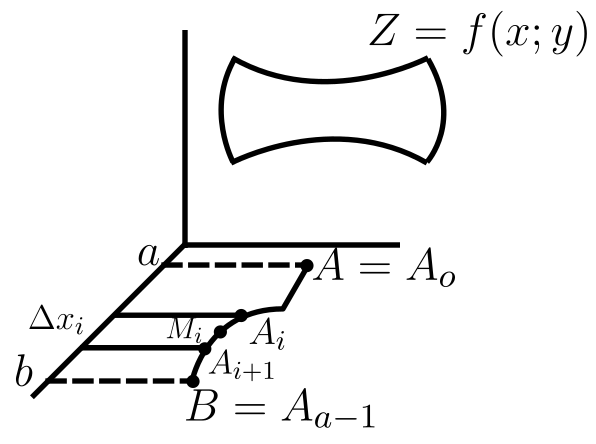
\includegraphics[scale=0.8]{8.3.1.png}
  \end{minipage}
  \hspace{1em}
  \begin{minipage}{0.65\textwidth}
    \begin{enumerate}
      \item R
      \item $M_i(\xi_i,\eta_i) \in \Delta l_i$
      \item $f(M_i)=f(\xi_i;\eta_i)$
      \item $\sum_{i=0}^{n-1}f(\xi_i;\eta_i)\Delta x_i=\sigma_R$
      \item $\lim_{\lambda_R \to 0}\sigma_R=\int_{(l)}f(x;y)dx$
    \end{enumerate}
  \end{minipage}
  \vspace{1em}
  \par
  \underline{Определение: } Если существует конечный предел суммы $\sigma_R$, не зависящей от способа
  разбиения кривой l и выбора (.) $M_i(\xi_i;\eta_i)$, то он называется криволинейным интегралом
  II рода от функции f(x;y) по кривой l\\
  \underline{Замечание:} Аналогично вводится\\
  \[\int_{(l)}f(x;y)dy\]\\
  Если вдоль кривой определенны функции $P(x;y),Q(x;y)$ и существует $\int_{(AB)}P(x;y)dx$ и
  $\int_{(AB)}Q(x;y)dy$, то $\int_{(AB)}P(x;y)dx+Q(x;y)dy$ называется криволинейным интегралом
  II рода общего вида.\\
  \underline{Замечание:} \[\int_{(AB)}f(x;y)dx=-\int_{(BA)}f(x;y)dx\]\\
  Аналогично вводится: \[\int_{(AB)}P(x;y;z)dx+Q(x;y;z)dy+R(x;y;z)dz\]
  \subsection{Существование и вычисление криволинейного интеграла II рода}
  \subsubsection*{Теорема 8.4.1}\label{th:8.4.1}
  \par\noindent
  Пусть кривая AB задана параметрически:\\
  $\begin{cases}
    x=\varphi(t) \hspace{20pt} \varphi(t),\psi(t) \text{ непрерывны } \forall t \in [a;b]\\
    y=\psi(t)
  \end{cases}$\\
  Пусть f=f(x;y) непрерывна вдоль кривой AB. $\varphi'(t)$ существует и непрерывна $\forall t \in [a;b]$.
  Тогда существует криволинейный интеграл $\int_{(AB)}f(x;y)dx=\int_{a}^{b}f(\varphi(t);\psi(t))\varphi'(t)dt$\\
  \underline{Доказательство:}
  \begin{adjustwidth}{1.5em}{1.5em}
    \begin{minipage}{0.45\textwidth}
      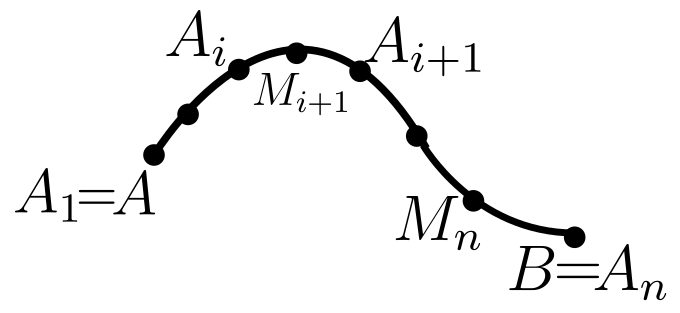
\includegraphics[scale=0.6]{8.4.1.png}
    \end{minipage}
    \hspace{1em}
    \begin{minipage}{0.55\textwidth}
      \begin{enumerate}
        \item Произведем разбиение R кривой (AB) точками $A_i(\varphi(t_i);\psi(t_i))$
        \item Выберем (.) $M_i(\varphi(\tau_i);\psi(\tau_i))$
        \item $\Delta x_i = \varphi(t_{i+1})-\varphi(t_i)=\int_{t_i}^{t_{i+1}}\varphi'(t)dt$
        \item $\sigma_R=\sum_{i=0}^{n-1}f(\varphi(\tau_i);\psi(\tau_i))\Delta x_i=\\=\sum_{i=0}^{n-1}
        f(\varphi(\tau_i);\psi(\tau_i))\int_{t_i}^{t_{i+1}}\varphi'(t)dt$
      \end{enumerate}
    \end{minipage}
    \vspace{1em}
    \par
  \end{adjustwidth}
  Рассмотрим правую часть: $\int f(\varphi(\tau_i);\psi(\tau_i))\varphi'(t)dt = \sum_{i=1}^{n}
    \int_{t_i}^{t_{i+1}}f(\varphi(\tau_i);\psi(\tau_i))\varphi'(t)dt=I$\\
  Рассмотрим $|\sigma_R-I|=\sum_{i=1}^{n} \int_{t_i}^{t_{i+1}} [f(\varphi(\tau_i);\psi(\tau_i))-
  f(\varphi(t);\psi(t))]\varphi'(t)dt \boxed{<}$\\
  Т.к. f(x;y) непрерывна вдоль кривой (AB)\\
  \[\forall \varepsilon >0 \exists \delta = \delta(\varepsilon):|\Delta t_i| < \delta \Rightarrow
  |f(\varphi(t_{i+1});\psi(t_{i+1}))-f(\varphi(t_i);\psi(t_i))|<\varepsilon\]\\
  или $\begin{matrix}
    [t_i;\tau_i] <[t_i;t_{i+1}]\\
    [\tau_i;t_{i+1}] < [t_i;t_{i+1}]
  \end{matrix} \hspace{20pt} \varphi'(t)$ непрерывна на $[t_i;t_{i+1}] \Rightarrow$ она ограничена на нём.\\
  Пусть $\forall i |\varphi'(t_i)|<L$\\
  \boxed{<} $|\varepsilon L \sum_{i=1}^{n} \int_{t_i}^{t_{i+1}}dt|=\varepsilon L(b-a)\Rightarrow \lim_{\lambda_R \to 0}\sigma_R=I$
  \begin{center}
    \textbf{Ч.т.д.}
  \end{center}
  Аналогично: \[\int_{(AB)}f(x;y)dy=\int_{a}^{b}f(\varphi(t);\psi(t))\psi'(t)dt\]\\
  Если кривая задана как y=y(x) \hspace{10pt} $a\leq x\leq b$. Тогда\\
  $\begin{cases}
    y=y(t)\\
    x=t
  \end{cases} \hspace{20pt} a\leq t\leq b \Rightarrow \int_{(AB)}f(x;y)dx =\int_{a}^{b} f(t;y(t))dt=
  |x=t|=\int_{a}^{b}f(x;y(x))dx$\\
  \underline{Замечание:} $\int_{(AB)}f(x;y)dx=0,$ если AB-прямоугольный отрезок || оси OY. Аналогично \\
  $\int_{(CD)}f(x;y)dy=0,$ если CD-прямоугольный отрезок || OX.\\
  Если L-замкнутый контур.\\
  \begin{minipage}{0.45\textwidth}
    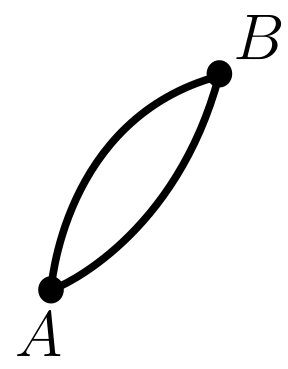
\includegraphics[scale=0.6]{8.4.2.png}
  \end{minipage}
  \hspace{1em}
  \begin{minipage}{0.25\textwidth}
    \[\int_{(l)}=\int_{(AB)}+\int_{(BA)}\]
  \end{minipage}
  \vspace{1em}
  \par
  Среди двух возможных обходов, L обход против часовой стрелки, причём за положительный обход. При обходе рассматриваемая область
  находится слева.
  \subsection{Вычисление площади криволинейной трапеции с помощью криволинейного интеграла.}
  \begin{minipage}{0.45\textwidth}
    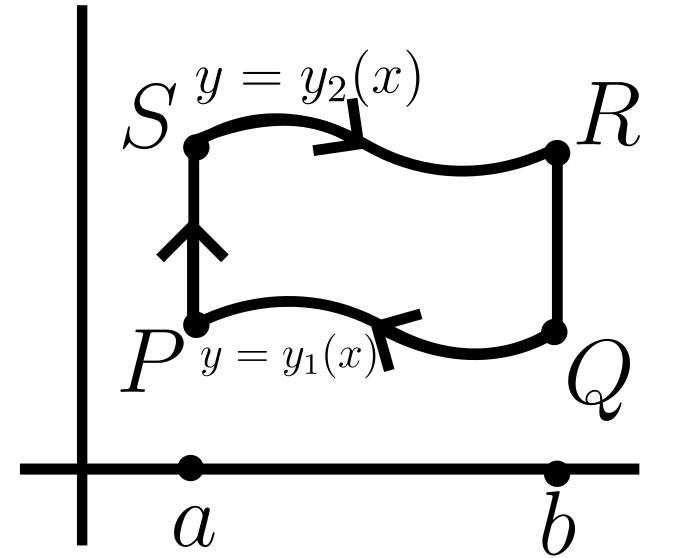
\includegraphics[scale=0.6]{8.5.1.png}
  \end{minipage}
  \hspace{1em}
  \begin{minipage}{0.55\textwidth}
    Найти S(PSRQ)\\
    \[S=\int_{a}^{b}y_2(x)dx-\int_{a}^{b}y_1(x)dx \boxed{=}\]\\
     \[\text{Рассмотрим} \int_{a}^{b}y_2(x)dx=\int_{(SR)}ydx\]\\
      \[\text{Рассмотрим}\int_{a}^{b}y_1(x)dx=\int_{(PQ)}ydx\]\\
    $\boxed{=} \int_{(SR)}ydx-\int_{(PQ)}ydx=\int_{(SR)}ydx+\int_{(QP)}ydx+$ \\ 
    \par
    $\int_{(PS)}ydx+\int_{(RQ)}ydx=\int_{(PSRQP)}ydx \boxed{=}$
  \end{minipage}
  \vspace{1em}
  \par
  Пусть L=(PQRSP) - контур взятый в положительном направлении. $\boxed{=}-\int_{(L)}ydx=S$\\
  Аналогично, если рассмотреть:
  \begin{flushleft}
    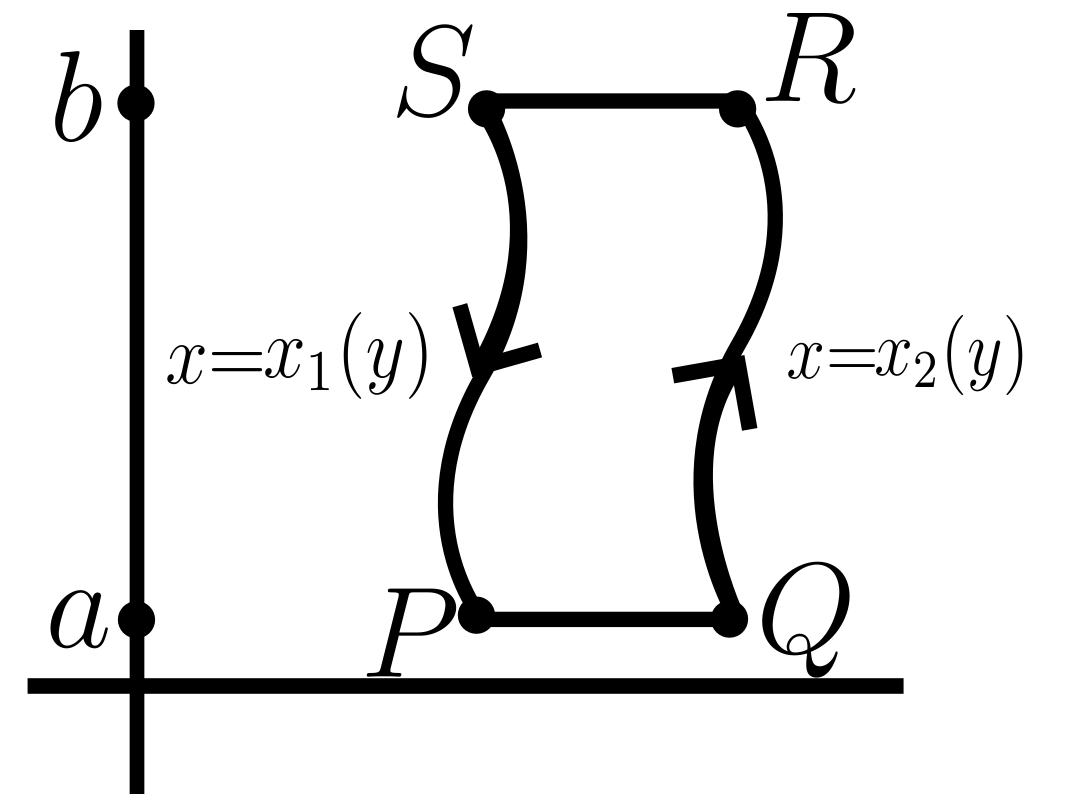
\includegraphics[scale=0.4]{8.5.2.png}
  \end{flushleft}
  То получим S=$\int_{(l)}xdy$\\
  Для произвольного замкнутого контура L\\
  \[\boxed{S=\frac{1}{2}\int_{(l)}xdy-ydx}\]
  \underline{Замечание:}
  \begin{flushleft}
      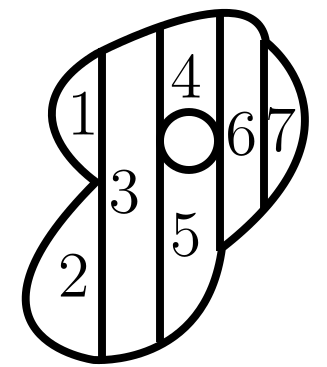
\includegraphics{8.5.3.png}
  \end{flushleft}
  \subsection{Связь между криволинейными интегралами I и II рода}
  Пусть кривая задана в виде $\overline{r}=\overline{r}(t) \hspace{20pt} a\leq t \leq b$\\
  \begin{flushright}
    $\overline{r}=\overline{r}(x(t^*);y(t^*))$
  \end{flushright}
  \begin{figure}[h!]
    \centering
    % Первая колонка (левая картинка)
    \begin{minipage}{0.45\textwidth}
        \centering
        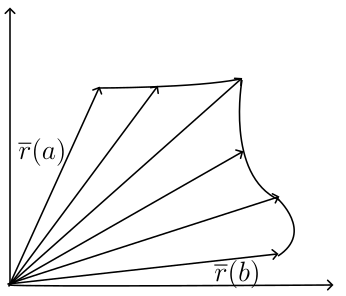
\includegraphics[width=\textwidth]{8.6.1.png} % путь к первой картинке
        \vspace{0.5em} % небольшой отступ между картинкой и текстом
        $\Delta \overline{r}=\overline{r}(t_o+\Delta t)-\overline{r}(t_0)$\\
        $\frac{\Delta \overline{r}}{\Delta t}=\frac{1}{\Delta t}*\Delta \overline{r}$\\
        $\lim_{\Delta t \to 0} \frac{\Delta \overline{r}}{\Delta t}=r(t_0)$\\
        $|\overline{r}'(t)|=l'(t)$
    \end{minipage}
    \hfill
    % Вторая колонка (правая картинка)
    \begin{minipage}{0.45\textwidth}
        \centering
        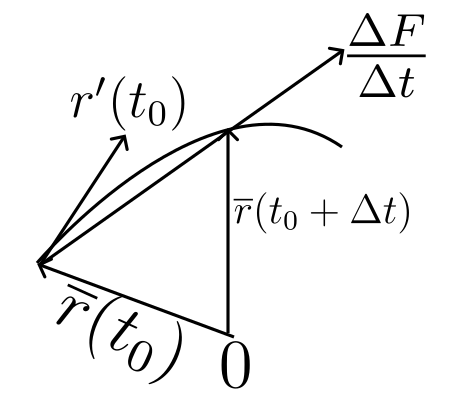
\includegraphics[width=\textwidth]{8.6.2.png} % путь ко второй картинке
        \vspace{0.5em} % небольшой отступ между картинкой и текстом
        $\overline{r}'(t)=\overline{x'(t);y'(t)}$\\
        $|\overline{r}'(t)=\sqrt{x'(t)^2+y'(t)^2}|$\\
        $dl=\sqrt{x'(t)^2+y'(t)^2}dt|:dt$\\
        $l'(t)=\sqrt{x'(t)^2+y'(t)^2}$
    \end{minipage}
  \end{figure}
  \par
  Пусть l-переменная длина дуги\\
  \[\frac{d \overline{r}}{dl} = \frac{d \overline{r}}{dt}* \frac{dt}{dl}=\frac{\frac{d \overline{r}}{dt}}{\frac{dl}{dt}}
  \hspace{20pt} \Big| \frac{d \overline{r}}{dt} \Big| = \Big| \frac{r'(t)}{l'(t)} \Big| = 1\]\\
  \underline{Замечание:} Если $|\overline{a}|=1 \Rightarrow \overline{a}(\cos(\alpha),\cos(\beta),\cos(\gamma))
  \hspace{20pt} \cos^2 \alpha+\cos^2 \beta+\cos^2 \gamma=1$\\
  \[\frac{d \overline{r}}{dl}=(\overline{\cos \alpha; \cos \beta})=(\overline{\frac{dx}{dl};\frac{dy}{dl}})\]\\
  \[\frac{dx}{dl}=\cos \alpha \hspace{20pt} dx=\cos \alpha dl\]\\
  \[\frac{dy}{dl}=\cos \beta \hspace{20pt} dy=\cos \beta dl\]\\
  Рассмотрим $\int_{(l)}f(x;y)dx=\int_{(l)}f(x;y)\cos \alpha dl$\\
  В общем случае $\int_{(l)}P(x;y;z)dx+Q(x;y;z)dy+R(x;y;z)dz=$\\
  \[\int_{(l)} [P(x;y;z)\cos \alpha + Q(x;y;z)\cos \beta + R(x;y;z)\cos \gamma]dl\]\\
  \subsection*{Физический смысл криволинейным интеграла II рода}
  Рассмотрим $\int_{(l)} Pdx+Qdy+Rdz$\\
  Пусть F(P;Q;R) - сила, под действием которой (.) перемещается по кривой l.\\
  d $\overline{S}(dx;dy;dz)$\\
  Рассмотрим $\overline{F}*\overline{ds}=A$\\
  Криволинейный интеграл II рода равен работе силы F по перемещению (.) по кривой l.
  \subsection{Условие независимости криволинейного интеграла от путей интегрирования.}
  Рассмотрим $\begin{matrix}
    P=P(x;y)\\
    Q=Q(x;y)
  \end{matrix}$\\
  Рассмотрим $\int_{(AB)}Pdx+Qdy \boxed{1}$\\
  Найти условия, при которых значение интеграла не зависит от вида кривой (AB) и однозначно определяется положением
  (.) A и (.) B\\
  Рассмотрим Pdx+Qdy \hspace{20pt} dF = $\frac{\delta F}{\delta x}dx + \frac{\delta F}{\delta y}dy$\\
  Если $P=\frac{\delta F}{\delta x} \hspace{20pt} Q=\frac{\delta F}{\delta y}$, то Pdx+Qdy является полными
  дифференциалом от некоторой F(x;y).\\
  \subsubsection*{Теорема 8.7.1}\label{th:8.7.1}
  \par\noindent
  $\Leftrightarrow$ чтобы Pdx+Qdy было в рассматриваемой области дифференциалом от некоторой функции 
  F(x;y)\\
  \underline{Доказательство:}
  \begin{adjustwidth}{1.5em}{1.5em}
    $\Rightarrow$ пусть \boxed{1} не зависит от путей интегрирования \\
    \hspace{1em}
    \begin{minipage}{0.55\textwidth}
      \[\int_{(AB)} Pdx+Qdy = \int_{(x_0;y_0)}^{(x_1;y_1)}Pdx+Qdy\]\\
      \[\text{Рассмотрим F(x;y)=}\int_{(x_0;y_0)}^{(x;y)}Pdx+Qdy\]
    \end{minipage}
    \vspace{1em}
    \begin{minipage}{0.45\textwidth}
      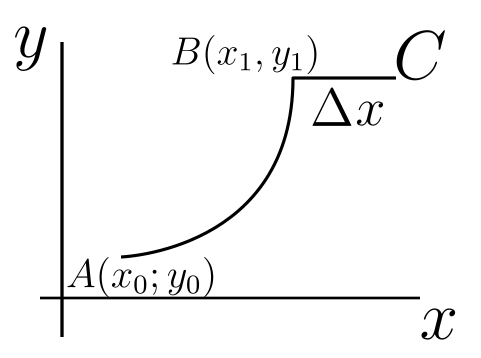
\includegraphics[scale=0.6]{8.7.1.png}
    \end{minipage}
    \par
    \[F(x;y)=\int_{(x_0;y_0)}^{(x_1;y_1)}Pdx+Qdy\]\\
    \[F(x_1+\Delta x;y_1)=\int_{(x_0;y_0)}^{(x_1+\Delta x;y_1)}Pdx+Qdy=\int_{(AB)}Pdx+qdy+
    \int_{(CD)}Pdx+Qdy\]\\
    Рассмотрим $F(x_1+\Delta x,y_1)-F(x_1;y_1)=\int_{(BC)}Pdx=\int_{x_1}^{x_1+\Delta x}P(x;y_1)dx=
    \Big| \text{\underline{Замечание:}} \int_{a}^{b}f(x)dx=f(\xi)(b-a)\Big| = \underset{\xi \in (x_1;x_1+\Delta x)}{P(\xi;y_1)}
    \Delta x = \underset{0<\theta<1}{P(x_1+\theta \Delta x;y_1)}\Delta x$\\
    \[\frac{F(x_1+\Delta x;y_1)-F(x_1;y_1)}{\Delta x} = P(x_1+\theta\Delta x;y_1)\]\\
    \[\lim_{\Delta x \to 0} \frac{F(x_1+\Delta x;y_1)-F(x_1;y_1)}{\Delta x}=\frac{\delta F}{\delta x} \Big|_{(x_1;y_1)}
    =P(x;y)\Big|_{(x_1;y_1)}\]\\
    \[\forall x \in D \hspace{20pt} \frac{\delta F}{\delta x}=P(x;y)\]\\
    Аналогично $\frac{\delta F}{\delta y}=Q(x;y)$\\
    $\Leftarrow$ Пусть Pdx+Qdy=$\frac{\delta F}{\delta x}+\frac{\delta F}{\delta y}dy$\\
    \[\int_{(l)}Pdx+Qdy= \begin{vmatrix}
      x=\varphi(t) & \varphi(a)=x_a & \varphi(b)=x_b\\
      y=\psi(t) & \psi(a)=y_a & \psi(b)=y_b  \\
      dx=\varphi'(t)dt\\
      dy=\psi'(t)dt
    \end{vmatrix} = \int_{a}^{b}[P(\varphi(t);\psi(t))\varphi'(t)+Q(\varphi(t);\psi(t))\psi'(t)]dt=\]\\
    \[=\int_{a}^{b}[\frac{\delta F}{\delta x}\varphi'(t)+\frac{\delta F}{\delta y}\psi'(t)]dt=\int_{a}^{b}
    \frac{dF(\varphi(t);\psi(t))}{dt}dt=F(\varphi(t);\psi(t))\Big|^b_a= F(x_b;y_b)-F(x_a;y_a)\]
    \begin{center}
      \textbf{Ч.т.д.}
    \end{center}
  \end{adjustwidth}
  \begin{center}
    Как установить, является ли выражение Pdx+Qdy полным дифференциалом?\\
    $Pdx+Qdy \overset{?}{=} dF$\\
    Если $\begin{matrix}
      P=\frac{\delta F}{\delta x} & Q=\frac{\delta F}{\delta y}\\
      \frac{\delta P}{\delta y}=\frac{\delta^2 F}{\delta y \delta x} & \frac{\delta Q}{\delta x}=\frac{\delta^2 F}{\delta x \delta y}
    \end{matrix} \Rightarrow \frac{\delta P}{\delta y}= \frac{\delta Q}{\delta x}$
  \end{center}
  
  
  \begin{minipage}{0.55\textwidth}
    \underline{Вопрос}: Как найти функцию F(x;y)?\\
    \[\int_{(l)}dF=F(x;y)+C\]\\
    Зафиксируем (.)$(x_0;y_0)$
  \end{minipage}
  \hspace{1em}
  \begin{minipage}{0.45\textwidth}
    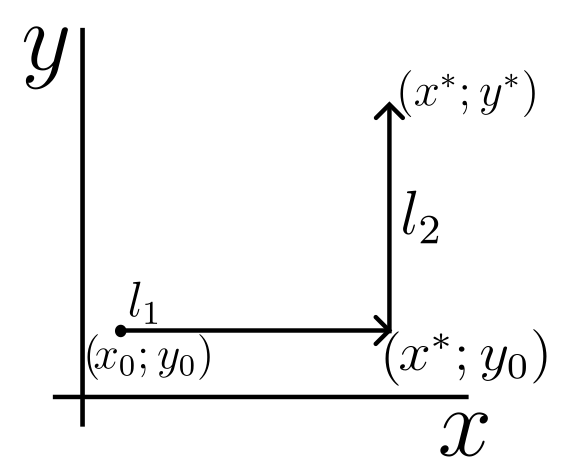
\includegraphics[scale=0.6]{8.7.2.png}
  \end{minipage}
  \vspace{1em}
  \par
  $\begin{matrix}
    \text{(x,y) - произвольная (.) области } & \hspace{20pt} & l_1: y=y_0 & dy=0\\
    \text{Обозначим её} (x^*;y^*) & \hspace{20pt} & l_2:x=x^x & dx=0
  \end{matrix}$\\
  \[\int_{(l)}Pdx+Qdy=\int_{(l_1)}Pdx+Qdy+\int_{(l_2)}Pdx+Qdy+C = \int_{x_0}^{x^*}P(x;y_0)dx+
  \int_{y_0}^{y^x}Q(x^*;y)dy+C=F(x^*;y^*)\]
  \subsection{Интеграл по замкнутому контуру}
  Рассмотрим $\int_{(l)}Pdx+Qdy$ L-замкнутый контур в положительном направлении.
  \begin{center}
    \underline{Вопрос:} При каких условиях интеграл по замкнутому контуру обращается в ноль?
  \end{center}
  \subsubsection*{Теорема 8.8.1}\label{th:8.8.1}
  \par\noindent
  Если $\int_{(AB)}Pdx+Qdy$ не зависит от пути интегрирования, то $\int_{(l)}Pdx+Qdy=0.$Верно и обратное утверждение.\\
  \begin{minipage}{0.25\textwidth}
    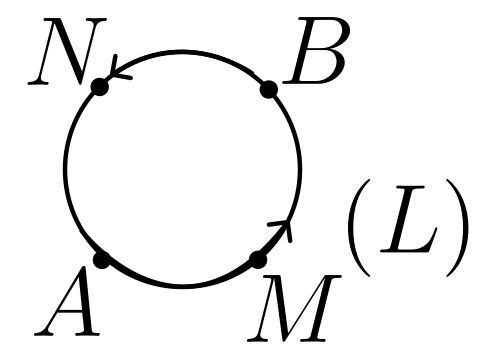
\includegraphics[scale=0.5]{8.8.1.png}
  \end{minipage}
  \hspace{1em}
  \begin{minipage}{0.75\textwidth}
    \underline{Доказательство:}\\
      $\Rightarrow : \int_{(AB)}Pdx+Qdy$ не зависит от пути интегрирования.\\
      $\int_{(AMB)}=\int_{(AMB)} \Rightarrow \int_{(AMB)}-\int_{(AMB)}=0 \Rightarrow
      \Rightarrow \int_{(AMB)}+\int_{(BNA)}=0 \Rightarrow \int_{(L)}=0$
  \end{minipage}
  \vspace{1em}
  \par
  $\Leftarrow:$ Пусть $\int_{(L)}=0$
  \begin{center}
    $\int_{(AMB)}+\int_{(BNA)}=0$\\
    $\int_{(AMB)}=-\int_{(BNA)}$\\
    $\int_{(AMB)}=\int_{(ANB)}$\\
  \end{center}
  \begin{center}
    \textbf{Ч.т.д.}
  \end{center}
  \underline{Замечание:} Существует область, для которых условие $\frac{\delta P}{\delta y}=\frac{\delta Q}{\delta x}$
  не является достаточным для того, чтобы криволинейный интеграл не зависел от пути интегрирования.\\
  \par
  \underline{Определение: } Область, для которой $\forall$ расположенный в ней замкнутый контур можно путём
  непрерывной деформации стянуть в (.), не выходя за пределы области, называется односвязной. В противном
  случаем - неодносвязной.\\
  \par
  \begin{minipage}{0.5\textwidth}
    односвязный\\
    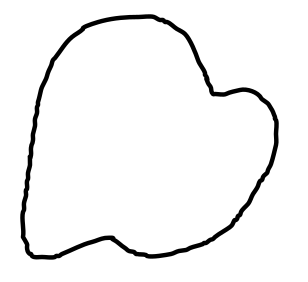
\includegraphics[scale=0.6]{8.8.2.png}
  \end{minipage}
  \hspace{1em}
  \begin{minipage}{0.5\textwidth}
      не односвязный\\
    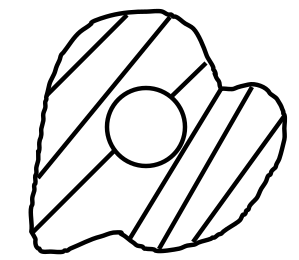
\includegraphics[scale=0.6]{8.8.3.png}
  \end{minipage}
  \vspace{1em}
  \par
  \textbf{Утверждение:} Для того, чтобы\\
  \[\oint_{(L)} Pdx+Qdy=0 \text{ необходимо, а в случае односвязной области достаточно, чтобы } \frac{\delta P}{\delta y}=\frac{\delta Q}{\delta x}\]
  Рассмотрим контур, имеющий внутри себя особую точку\\
  \textbf{Утверждение:} Пусть $\frac{\delta P}{\delta y}=\frac{\delta Q}{\delta x}$. Тогда
  \begin{enumerate}
    \item $\oint_{L}Pdx+Qdy$ может быть отличным от нуля.
    \item Все интегралы взятые в "+" направлении, по $\forall$ замкнутому контуру, будут равны между собой.
  \end{enumerate}
  \underline{Доказательство:}\\
  2)
  \begin{minipage}{0.45\textwidth}
    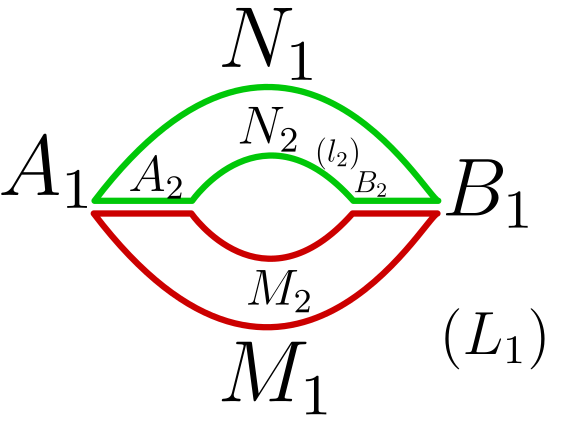
\includegraphics[scale=0.6]{8.8.4.png}
  \end{minipage}
  \hspace{1em}
  \begin{minipage}{0.55\textwidth}
    Рассмотрим \\
    \[\begin{matrix}
      \int_{(A_1M_1B_1)}+\int_{B_1B_2}+\int_{B_2M_2A_2}+\int_{A_1A_1} = 0\\
      \int_{B_1N_1A_1}+\int_{A_1A_2}+\int_{A_2N_2B_2}+\int_{B_2B_1} =0 
    \end{matrix} \Bigg\} \Rightarrow\] 
    \[\Rightarrow \int_{A_1M_1B_1N_1A_1} + \int_{B_2M_2N_2N_2B_2} =0 \]
    \[\int_{A_1M_1B_1N_1A_1}=-\int_{B_2M_2A_2N_2B_2}\]
    \[\int_{(l_1)}=\int_{(l_2)}\]
  \end{minipage}
  \vspace{1em}
  \begin{center}
    \textbf{Ч.т.д.}
  \end{center}
  Рассмотрим $\oint_{(L)} Pdx+Qdy=\sigma$\\
  \begin{minipage}{0.45\textwidth}
    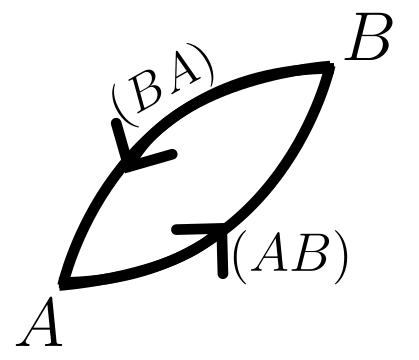
\includegraphics[scale=0.6]{8.8.5.png}
  \end{minipage}
  \hspace{1em}
  \begin{minipage}{0.4\textwidth}
    \[\int_{(AB)}Pdx+Qdy+\int_{(BA)}Pdx+Qdy=n\sigma\]
    \[\int_{(AB)}Pdx+Qdy=\int_{(AB)}Pdx+Qdy+n\sigma\]
  \end{minipage}
  \vspace{1em}
  \par
  То есть интеграл зависит от пути интегрирования. В смысле прибавления кратного числа к циклической
  постоянной.\\
  Присоединив к кривой AB некоторое число петель, окружающих особую (.), можно добиться, чтобы криволинейный
  интеграл принял значение, близкое к заданному.\\
  \underline{Пример:} $\oint_{(L)} \frac{xdy-ydx}{x^2+y^2} \boxed{=} \hspace{20pt} L:x^2+y^2=a^2, r=a$\\
  \begin{minipage}{0.2\textwidth}
    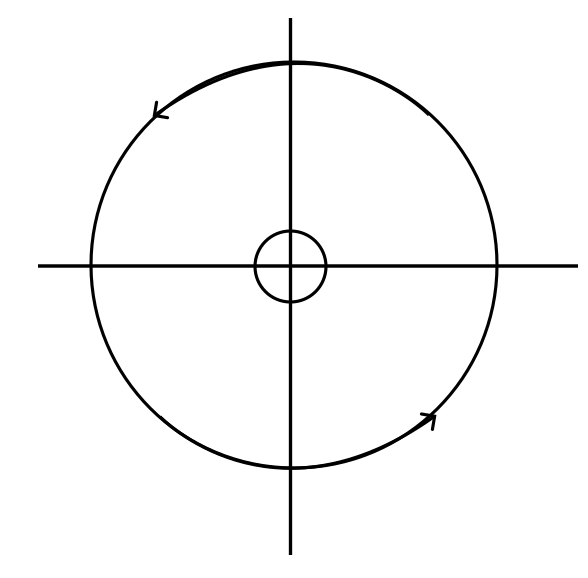
\includegraphics[scale=0.4]{8.8.6.png}
  \end{minipage}
  \hspace{1em}
  \begin{minipage}{0.8\textwidth}
    $P=\frac{-y}{x^2+y^2} \hspace{20pt} Q=\frac{x}{x^2+y^2} \hspace{10pt}$
    $\begin{matrix}
      x=r(\varphi)\cos(\varphi)=a\cos(\varphi) & dx=-a\sin(\varphi)d\varphi\\
      y=a\sin(\varphi) & dy=a\cos(\varphi)d\varphi
    \end{matrix}$
  \end{minipage}
  \vspace{1em}
  \par
  \[\boxed{=} \int_{0}^{2\pi} \frac{a^2\cos^2(\varphi)+a^2\sin^2(\varphi)}{a^2}d\varphi = 
  \int_{0}^{2\pi}d\varphi=\varphi \Big|^{2\pi}_0 = 2\pi = \sigma\]
  \begin{center}
    В общем случае $\oint_{(L)} Pdx+Qdy=n_1\sigma_1+n_2\sigma_2+\dots+n_k\sigma_k$
  \end{center}
  \subsection{Трёхмерный случай}
  Рассмотрим $\int_{(AB)}Pdx+Qdy+Rdz$\\
  Он не зависит от пути интегрирования, если существует F(x;y;z):
  \[\frac{\delta F}{\delta x}=P;\frac{\delta F}{\delta y}=Q;\frac{\delta F}{\delta Z}=R\]

  \[\text{Пусть существует непрерывные производные } \frac{\delta P}{\delta y};
  \frac{\delta P}{\delta z};\frac{\delta Q}{\delta x};\frac{\delta Q}{\delta z}
  ;\frac{\delta R}{\delta x};\frac{\delta R}{\delta y}\]

  \[\frac{\delta P}{\delta y}=\frac{\delta^2 F}{\delta y \delta x};
  \frac{\delta P}{\delta z}=\frac{\delta^2 F}{\delta z \delta x};
  \frac{\delta Q}{\delta x}=\frac{\delta^2 F}{\delta x \delta y};
  \frac{\delta Q}{\delta z}=\frac{\delta^2 F}{\delta z \delta y};
  \frac{\delta R}{\delta x}=\frac{\delta^2 F}{\delta x \delta z};
  \frac{\delta R}{\delta y}=\frac{\delta^2 F}{\delta y \delta z}\]

  \[\begin{matrix}
    \frac{\delta P}{\delta y} = \frac{\delta Q}{\delta x}\\
    \par \\
    \frac{\delta P}{\delta z} = \frac{\delta R}{\delta x}\\
    \par \\
    \frac{\delta Q}{\delta z} = \frac{\delta R}{\delta y}
  \end{matrix} \Bigg\} \text{- условие независимости криволинейного интеграла от пути интегрирования}\] 
  $P=\frac{\delta F}{\delta x}$\\
  Рассмотрим $\int_{x_0}^{x} P(x;y;z)dx=\int_{x_0}^{x}\frac{\delta F}{\delta x}dx = F(x;y;z)-F(x_0;y;z)$\\
  Зафиксируем $x_0. \int_{y_0}^{y}Q(x_0;y;z)dy=\int_{y_0}^{y}\frac{\delta F}{\delta y|_{x=x_0}}
  dy=F(x_0;y;z)-F(x_0;y_0;z)$\\
  Зафиксируем $x_0,y_0. \int_{z_0}^{z}R(x;y;z)dz=\int_{z_0}^{z}\frac{\delta F}{\delta z |_{x_0,y_0}}dz=
  F(x_0;y_0;z)-F(x_0;y_0;z_0)$
  \[F(x;y;z)=\int_{x_0}^{x}P(x;y;z)dx+\int_{y_0}^{y}Q(x_0;y;z)dy+\int_{z_0}^{z}R(x_0;y_0;z)dz+\equalto{F(x_0;y_0;z_0)}{C}\]
  \subsection{Кратные интегралы. Двойной интеграл в прямоугольной области.}
  \begin{minipage}{0.25\textwidth}
    Рассмотрим P: $\begin{matrix}
      a\leq x \leq b\\
      c \leq y \leq d
    \end{matrix}$
  \end{minipage}
  \hspace{1em}
  \begin{minipage}{0.45\textwidth}
    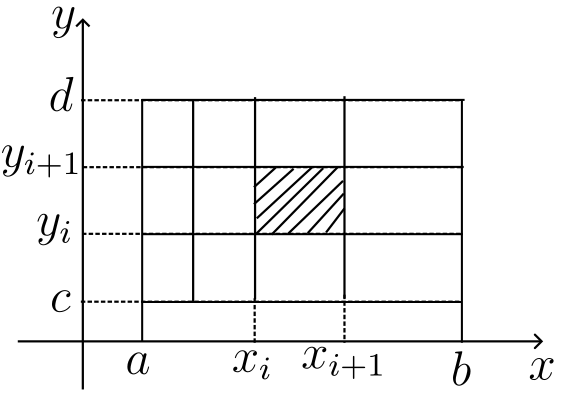
\includegraphics[scale=0.6]{8.10.1.png}
  \end{minipage}
  \vspace{1em}
  \par
  \begin{enumerate}
    \item R: $\begin{matrix}
      a=x_0 < x_1 < \dots < x_n =b\\
      c=y_0 <y_1 < \dots < y_n =d
    \end{matrix}$
    \item Выберем в каждом элементарном $P_{ij}$ произвольную (.) $(\xi_i;\eta_i)$
    \item Рассмотрим Z=f(x;y). Вычислим $f(\xi_i;\eta_i)$
    \item Вычислим $f(\xi_i;\eta_i)S_{P_{ij}}$
    \item Вычислим $\sum_{i=0}^{n-1} \sum_{j=0}^{m-1} f (\xi_i;\eta_i)S_{P_{ij}}$
    \item Обозначим $\lambda_R = max(d_{ij})$
    \item $\lim_{\lambda_R \to 0}\sigma_R=\iint_P f(x;y)dxdy$
  \end{enumerate}
  \underline{Определение: } Если существует конечный $\lim_{\lambda_R \to 0} \sigma_R$, не зависящий
  от способа разбиения R и выбора (.) $(\xi_i;\eta_i)$, то он называется двойным интегралом от f(x;y)
  по прямоугольнику P.\\
  \par\noindent
  \underline{Определение: } I называется двойным интегралом от f(x;y) по P, если 
  \[\forall \varepsilon > 0 \exists \delta =\delta(\varepsilon): \lambda_r < \delta \Rightarrow |I-\sigma_R| < \varepsilon\]

  \subsection{Суммы Дарбу}
  \[\overline{S}=\sum_{i=0}^{n-1} \sum_{j=0}^{m-1} M_{ij}\Delta x_i \Delta y_i = \sum_{i=1}^{n-1} \sum_{j=0}^{n-1}M_{ij}\Delta P_{ij}\]
  \[\underline{S}=\sum_{i=0}^{n-1} \sum_{j=0}^{m-1} m_{ij}\Delta x_i \Delta y_i = \sum_{i=1}^{n-1} \sum_{j=0}^{n-1}m_{ij}\Delta P_{ij}\]
  \[m_{ij} \leq f(x;y) \leq M_{ij} \hspace{20pt} \forall(x;y)\in P_{ij}\]
  \[M_{ij}=\underset{(x;y) \in \Delta P_{ij}}{sup f(x;y)} \hspace{20pt} m_{ij}=\underset{(x;y) \in \Delta P_{ij}}{inf f(x;y)} \]
  \subsection*{Свойства}
  \begin{enumerate}
    \item $\underline{S}\leq \sigma_R \leq \overline{S}, \forall R$
    \item Пусть $R \sqsubset R'$\\
    $\overline{S_{R'}}\leq \overline{S_{R}} \hspace{20pt} \underline{S_{R'}}\geq \underline{S_{R}}$
    \item $\forall R_1,R_2 \hspace{20pt} \underline{S_{R_1}}\leq \overline{S_{R_2}}$
    \item Множество верхних сумм Дарбу ограничено снизу.\par
    Множество нижних сумм Дарбу ограниченно сверху.\\
    $I_*=\underset{R}{sup \{\underline{S}\}} \hspace{20pt} I^*=\underset{R}{inf \{\underline{S}\}}$
    \item Th. о существовании интеграла\\
    f(x;y) интегрируема на P $\Leftrightarrow \lim_{\lambda_R \to 0} (\overline{S_R}-\underline{S_R})=0$\\
    $I_*=I^*=I$
  \end{enumerate}

  \subsection{Двойной интеграл в произвольной области}
  Пусть $\underset{\text{(квадратируема по Жордану)}}{\text{область D имеет конечную площадь}}$\\
  \begin{minipage}{0.45\textwidth}
    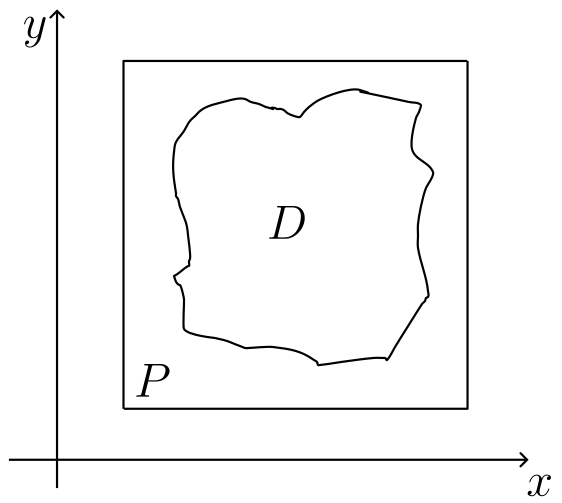
\includegraphics[scale=0.7]{8.12.1.png}
  \end{minipage}
  \hspace{1em}
  \begin{minipage}{0.55\textwidth}
    Пусть F(x;y)=$\begin{cases}
      f(x;y) & (.)(x;y) \in D\\
      0 & (.)(x;y) \not \in D
    \end{cases}$\\
    Если F(x;y) интегрируема в Р, то существует: \[\iint_{P} F(x;y)dxdy \]
    \[\iint_{P} F(x;y dxdy=\iint_{D} f(x;y)dxdy)\]
  \end{minipage}
  \vspace{1em}
  \par
  \begin{minipage}{0.45\textwidth}
    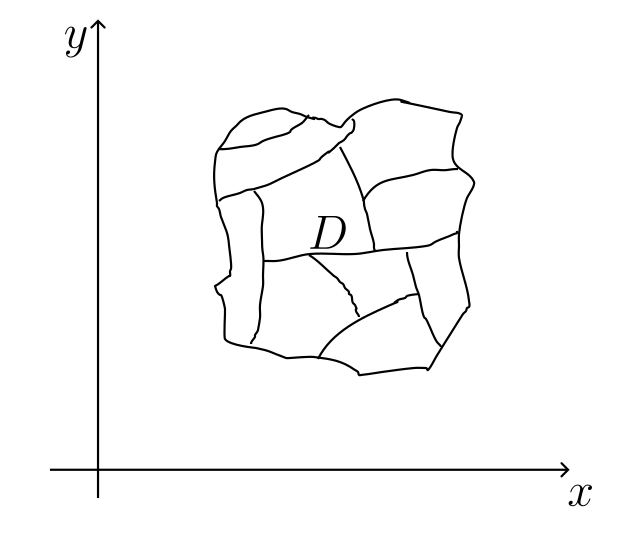
\includegraphics[scale=0.6]{8.12.2.png}
  \end{minipage}
  \hspace{1em}
  \begin{minipage}{0.55\textwidth}
    \begin{enumerate}
      \item Разобьем D спрямляемыми кривыми(кривая имеющая конечную длину)
      \item Выберем (.) $((\xi_i;\eta_i)) \in D_i$
      \item Вычислим $f((\xi_i;\eta_i))\Delta D_i$
      \item Составим $\sigma_R=\sum_{i=0}^{n-1}f((\xi_i;\eta_i))\Delta D_i$
      \item Пусть $\lambda_R = \underset{M_1,M_2 \in D_i}{\max \rho(M_1,M_2)}$
      \item Вычислим $\lim_{\lambda_R \to 0}\sigma_R=\iint_{D}f(x;y)dxdy$
    \end{enumerate}
  \end{minipage}
  \vspace{1em}
  \break
  \underline{Определение: } Если существует конечный предел $\sigma_R$, при $\lambda_R \to 0$, не
  зависящий от способа разбиения области D и выбора (.) $(\xi_i;\eta_i)$, то он называется двойным
  интегралом от функции f(x;y) по области D\\
  \subsection*{Свойства:}
  \begin{enumerate}
    \item $\iint_D dxdy=S_p$
    \item Пусть $D=D_1 \lor D_2: D_1\land D_2 =0$\\
    Если f(x;y) интегрируема в D, то она интегрируема в $D_1$ и $D_2$
    \[\iint_D f(x;y) dxdy=\iint_{D_1}f(x;y)dxdy+\iint_{D_2}f(x;y)dxdy\]
    \item Если f и g интегрируемы в D, то существует 
    \[\iint_D [\alpha f(x;y)+ \beta g(x;y)]dxdy=\alpha \iint_D f(x;y)dxdy+ \beta \iint_D g(x;y)dxdy\]
    \item Пусть f,g $\geq 0$ в D и $\forall (.) (x;y) \in D f\leq g$\\
    \[\iint_D f(x;y)dxdy\leq \iint_D g(x;y)dxdy\]
    \item Пусть f>0 $D_1 \subset D_2$
    \[\iint_{D_1} f(x;y)dxdy<\iint_{D_2} f(x;y)dxdy\]
    \item Если f интегрируема в D, то |f| тоже интегрируема в D
    \[\Big| \iint_D f(x;y)dxdy \Big| \leq \iint|f(x;y)|dxdy\]
    \item  
    \subsubsection*{Теорема о среднем}\label{th:8.12.1}
    \par\noindent
    Пусть f и g ограничены и интегрируемы в D, g не меняет знак в D
    \[m\leq f(x;y)\leq M. \text{ Тогда существует }\lambda: m\leq \lambda \leq M: 
    \iint_D f(x;y) g(x;y)dxdy=\lambda \iint_D g(x;y)dxdy\]\\
    Если дополнить f(x;y) непрерывна в D, то существует
    \[(.) (\xi_i;\eta_i) \in D: \iint_D f(x;y)dxdy=f (\xi_i;\eta_i) \Delta D\]
  \end{enumerate}
  \subsection{Вычисление двойного интеграла(сведение двойного интеграла к повторному)}
  Пусть f(x;y) задана в P = [a;b]x[c;d]. $\hspace{20pt}$ Рассмотрим F(x)=$\int_{a}^{c}f(x;y)dy$
  \subsubsection*{Теорема 8.13.1}\label{th:8.13.1}
  \par\noindent
  Если f(x;y) непрерывна в P, то F(x) непрерывна на [a;b]\\
  \underline{Доказательство:}
  \begin{adjustwidth}{1.5em}{1.5em}
    Рассмотрим $F(x+\Delta x)-F(x)=\int_{c}^{d}[f(x+\Delta x)-f(x;y)]dy \hspace{20pt} x,x+\Delta x \in [a;b]$\\
    По условию f(x;y) непрерывна в P $\Rightarrow f(x;y)$ будет равномерно непрерывна в P. \[\forall f(x;y)
    ,(x+\Delta x;y)\in P: |\Delta x|<\delta \Rightarrow |f(x+\Delta x;y)-f(x;y)|< \frac{\varepsilon}{d-c}\]\\
    То есть F(x) непрерывна в (.) x. Так как x-произвольная (.) $\in [a;b],$то F(x) непрерывна на [a;b]
    \begin{center}
      \textbf{Ч.т.д.}
    \end{center}
  \end{adjustwidth}
  \subsubsection*{Теорема 8.13.2}\label{th:8.13.2}
  \par\noindent
  Пусть $\iint_P f(x;y)dxdy$ существует. Тогда 
  \[\iint_D f(x;y)dxdy=\int_{a}^{b}dx \int_{c}^{d} f(x;y)dy=\int_{c}^{d}dy \int_{a}^{b}f(x;y)dx\]
  \underline{Доказательство:}
  \begin{adjustwidth}{1.5em}{1.5em}
    R:$\begin{cases}
      a:x_0<x_1<\dots<x_n=b & m_{ij}\leq f(x;y) \leq M_{ij} \forall (x;y) \in P_{ij} (*)\\
      c=y_0<y_1<\dots<y_k=d
    \end{cases}$\\
    Зафиксируем x=$\xi_i \in [x_i;x_{i+1}]$ и проинтегрируем (*) по переменной y
    \[\int_{y_j}^{y_{j+1}}m_{ij}dy \leq \int_{y_j}^{y_{j+1}}f(\xi_i;y)dy \leq \int_{y_j}^{y_{j+1}} M_{ij}dy\]
    \[m_{ij}\Delta y_j \leq \int_{y_j}^{y_{j+1}} f (\xi_i;y)dy \leq M_{ij}\Delta y_j\]
    \[\sum_{j=0}^{k-1} m_{ij}\Delta y_j \leq \sum_{j=0}^{k-1}\int_{y_j}^{y_{j+1}}f (\xi_i;y)dy
    \leq \sum_{j=0}^{k-1} M_{ij}\Delta y_j \Big| *\Delta x_i \text{ и проинтегрируем по } 
    i=\overline{0,n-1}\]
    \[\sum_{i=0}^{n-1}\sum_{j=0}^{k-1} m_{ij}\Delta x_j \Delta y_j \leq \sum_{i=0}^{n-1}
    [\int_{c}^{d} \equalto{f (\xi_i;y)}{I(\xi_i)}]\Delta x_i \leq 
    \sum_{i=0}^{n-1} \sum_{j=0}^{k-1} M_{ij} \Delta x_i \Delta y_j\]
    \[\text{При }\lambda_R \to 0: m_{ij},M_{ij} \rightarrow I= \iint_P f(x;y) dxdy\]
    %TODO:Найти способ как написать стрелку под текстом, пикча в Images лежит 
    Тогда $\iint_P f(x;y) dxdy = \lim_{\lambda_R \to 0} \sum_{i=0}^{n-1}I(\xi_i)\Delta x_i =
    \int_{a}^{b}I(x)dx=\int_{a}^{b}dx \int_{c}^{d}f(x;y)dy$\\
    Аналогично $\iint_P f(x;y)dxdy=\int_{c}^{d}dy \int_{a}^{b}f(x;y)dx$
    \begin{center}
      \textbf{Ч.т.д.}
    \end{center}
  \end{adjustwidth}
  \subsection{Вычисление двойного интеграла по произвольной области}
  \subsubsection*{Теорема 8.14.1}\label{th:8.14.1}
  \par\noindent
  Пусть $y_1(x)$ и $y_2(x)$ непрерывна на [a;b].\\
  Рассмотрим D:
  $\begin{cases}
    a\leq x\leq b\\
    y_1(x)\leq y \leq y_2(x)
  \end{cases}$\\
  Если f(x;y) задана в D и $\forall x \in [a;b]$ она интегрируема по y на $[y_1(x);y_2(x)]$ и
  f(x;y) непрерывна в D, то F(x) = $\int_{y_1(x)}^{y_2(x)}f(x;y)dy$ непрерывна на [a;b].\\
  \underline{Доказательство:}
  \begin{adjustwidth}{1.5em}{1.5em}
    Замена $y=y_1(x)+(y_2(x)-y_1(x))t \hspace{20pt} 0\leq t\leq 1 \hspace{20pt} dy=(y_2(x)-y_1(x))dt$
    \[F(x)=\int_{0}^{1} \underbrace{f(x;y_1(x)+(y_2(x)-y_1(x))t)(y_2(x)-y_1(x))}_{g(x;t)}dt=
    \int_{0}^{1}g(x;t)dt\]
    \begin{center}
      g(x;t) определена в прямоугольнике\\
      $a\leq x\leq b$\\
      $0\leq t\leq1$
    \end{center} 
    Тогда F(x) непрерывна по \hyperref[th:8.13.1]{Теореме 8.13.1}
    \begin{center}
      \textbf{Ч.т.д.}
    \end{center}
  \end{adjustwidth}
  \subsubsection*{Теорема 8.14.2}\label{th:8.14.2}
  \par\noindent
  Пусть f(x;y) интегрируема и непрерывна в D и $\forall x \in [a;b]$ прямая || OY пересекает границу
  D не более чем в $2^x$(.). То есть область D задана в виде D:
  $\begin{cases}
    a\leq x\leq b\\
    y_1(x)\leq y\leq y_2(x)
  \end{cases}$.\\
  Тогда:
  \[\iint_D f(x;y)dxdy = \int_{a}^{b}dx \int_{y_1(x)}^{y_2(x)}dy\]
  \underline{Замечание:} Аналогично можно рассмотреть: $\iint_D f(x;y)dxdy = \int_{c}^{d}dy
  \int_{x_1(y)}^{x_2(y)}f(x;y)dx$, если прямая || OX пересекает D не более чем в $2^x$(.).\\
  \underline{Замечание:}Если контур пересекается не более чем в $2^x$(.) как прямыми || OY,
  так и || OX, то справедливы обе формулы.\\
  \underline{Замечание:} Если контур не подходит ни под один случай, то его разбивают на $D_1,D_2,\dots$\\
  \underline{Доказательство:}
  \begin{adjustwidth}{1.5em}{1.5em}
    F(x) $\overset{\text{(на [a;b])}}{\text{непрерывна}}$ по \hyperref[th:8.14.1]{Теореме 8.14.1}. Тогда F(x)
    интегрируема на [a;b]. То есть, существует: \[\int_{a}^{b}F(x)dx=\int_{a}^{b}dx \int_{y_1(x)}^{y_2(x)}
    f(x;y)dy\]\\
    Введем разбиение:
    $\begin{cases}
      \vspace{2pt}
      x_i = a + \frac{b-a}{k}i \\
      \vspace{2pt}
      x_i-x_{i+1}=\frac{b-1}{k} \\
      i=\overline{1,k}
    \end{cases}$\\
    Введем вспомогательные функции:
    $\begin{cases}
      \vspace{2pt}
      \varphi_0(x)=y_1(x)\\
      \vspace{2pt}
      \varphi_1(x)=y_1(x)+\frac{y_2(x)-y_1(x)}{k}i\\
      \vdots\\
      \varphi_j(x)=y_1(x)+\frac{y_2(x)-y_1(x)}{k}j\\
      \vspace{2pt}
      \varphi_k(x)=y_1(x)+\frac{y_2(x)-y_1(x)}{k}k
    \end{cases}$\\
    Получим разбиение: 
    \[E^{k}_{ij}=
    \begin{cases}
      x_{i-1}\leq x \leq x_i\\
      \varphi_{j-1}\leq y\leq \varphi_j
    \end{cases} \hspace{20pt} i,j = \overline{1,k}\]
    \[m_{ij}=\underset{(x,y) \in E_{ij}^k}{\inf f(x;y)} \hspace{20pt} M_{ij}=\underset{(x,y) \in E_{ij}^k}{\sup f(x;y)}\]\\
    \[ \text{Рассмотрим} 
    \int_{a}^{b}dx+\int_{y_1(x)}^{y_2(x)}f(x;y)dy =
    \sum_{i=1}^{k} \int_{x_{i-1}}^{x_i}dx \sum_{j=1}^{k} \int_{\varphi_{j-1}}^{\varphi_j}f(x;y)dy =
    \sum_{i=1}^{k}\sum_{j=1}^{k} \int_{x_{i-1}}^{x_i} dx\int_{\varphi_{j-1}}^{\varphi_j}f(x;y)dy \leq\]
    \[\leq \sum_{i=1}^{k}\sum_{j=1}^{k} M_{ij} \int_{x_{i-1}}^{x_i}dx \int_{\varphi_{j-1}}^{\varphi_j}dy=
    \sum_{i=1}^{k}\sum_{j=1}^{k} M_{ij} M_{ij} \int_{x_{i-1}}^{x_i}dx[\varphi_j(x)-\varphi_{j_1}(x)]=
    \sum_{i=1}^{k}\sum_{j=1}^{k} \overbrace{\Delta E_{ij}^k}^{\text{S площадь}}=
    \overline{S}_R\]\\
    Аналогично $\int_{a}^{b}dx \int_{y_1(x)}^{y_2(x)}f(x;y)dy \geq \underline{S}_R$\\
    Получим $\underline{S}_R \leq \int_{a}^{b}dx \int_{y_1(x)}^{y_2(x)} f(x;y) dy \leq \overline{S}_R$
    %TODO переделать стрелки, лежит images peredelat2
    \begin{center}
      \textbf{Ч.т.д.}
    \end{center}
  \end{adjustwidth}
  \subsection{Формула Грина}
  \begin{minipage}{0.45\textwidth}
    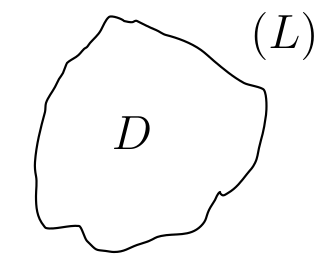
\includegraphics[scale=1]{8.15.1.png}
  \end{minipage}
  \hspace{1em}
  \begin{minipage}{0.55\textwidth}
    \[\oint_{L}Pdx+Qdy\]
  \end{minipage}
  \vspace{1em}
  \par

  \begin{minipage}{0.45\textwidth}
    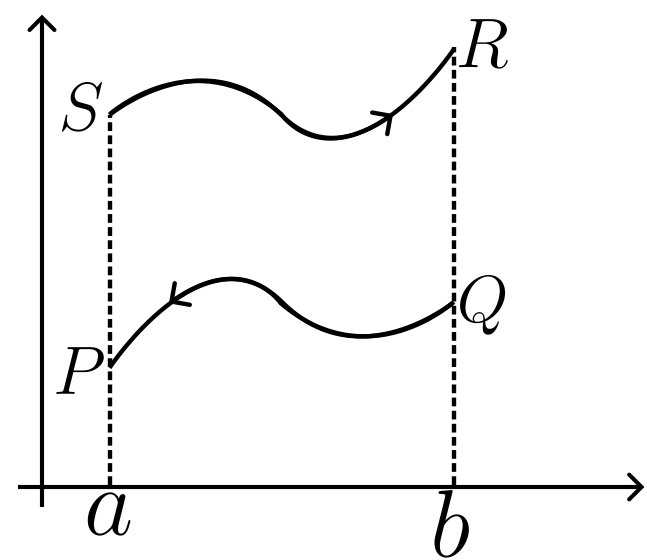
\includegraphics[scale=0.6]{8.15.2.png}
  \end{minipage}
  \hspace{1em}
  \begin{minipage}{0.55\textwidth}
    Рассмотрим 
    $\begin{cases}
      PQ:y=y_1(x)\\
      SR: y=y_2(x)\\
      a\leq x \leq b\\
      PS|OY, QR||OY
    \end{cases}$\\
  \end{minipage}
  \vspace{1em}
  \par
  Пусть в области D задана P(x;y). P(x;y) непрерывна $\frac{\delta P}{\delta y}$ непрерывна.
  \[\text{Рассмотрим }\] \[ \iint_D \frac{\delta P}{\delta y}dxdy= 
  \int_{a}^{b}dx \int_{y_1(x)}^{y_2(x)} \frac{\delta P}{\delta y}dy=
  \int_{a}^{b}dx \Big[P(x;y)\Big|_{y_1(x)}^{y_2(x)}\Big]=
  \int_{a}^{b}dx \Big[P(x;y_2(x))-P(x;y_1(x))\Big] \boxed{=}\]
  \[\text{Рассмотрим} \int_{a}^{b}P(x;y_2(x))dx=\int_{(SR)}P(x;y)dx\]
  \[\text{Рассмотрим} \int_{a}^{b}P(x;y_1(x))dx=\int_{(PQ)}P(x;y)dx=-\int_{(QP)}P(x;y)dx\]
  \[\boxed{=} \int_{(SR)}P(x;y)dx +\int_{(QP)}P(x;y)dx+\int_{(RQ)}P(x;y)dx+\int_{(PS)}P(x;y)dx \boxed{=}\]
  Пусть L-контур в положительном направлении.
  \[\boxed{=} - \int_{(L)}P(x;y)dx\]\\
  \break
  Аналогично:\\
  \par
  \begin{minipage}{0.45\textwidth}
    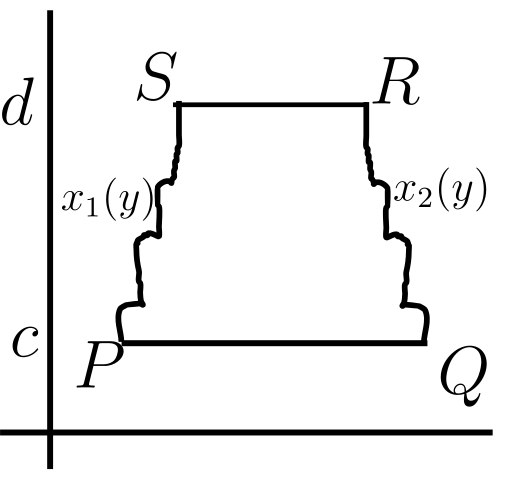
\includegraphics[scale=0.8]{8.15.3.png}
  \end{minipage}
  \hspace{1em}
  \begin{minipage}{0.55\textwidth}
    \[0,\frac{\delta Q}{\delta x} \text{непрерывна в D}\]
    \[\iint_P \frac{\delta Q}{\delta x}dxdy=\dots=\int_{(L)} Q(x;y)dy\] 
  \end{minipage}
  \vspace{1em}
  \par
  \begin{center}
    Если область D удовлетворяет обоим случаям, тогда справедлива формула:
    \[\boxed{\int_{(L)}Pdx+Qdy=\iint_D \Big[ \frac{\delta Q}{\delta x}-\frac{\delta P}{\delta y}\Big]dxdy}\]
  \end{center}
  \break
  \subsection{Замена переменных в двойном интеграле}
  \subsection*{I Преобразование плоских областей.}
  Рассмотрим 2 прямоугольных СК: xy и $\xi \eta$\\
  \begin{minipage}{0.5\textwidth}
    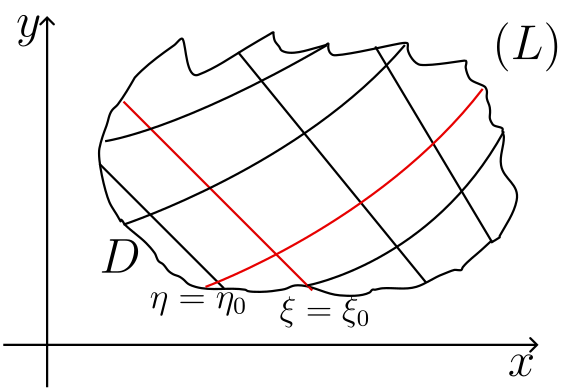
\includegraphics[scale=0.8]{8.16.1.png}
  \end{minipage}
  \hspace{1em}
  \begin{minipage}{0.5\textwidth}
    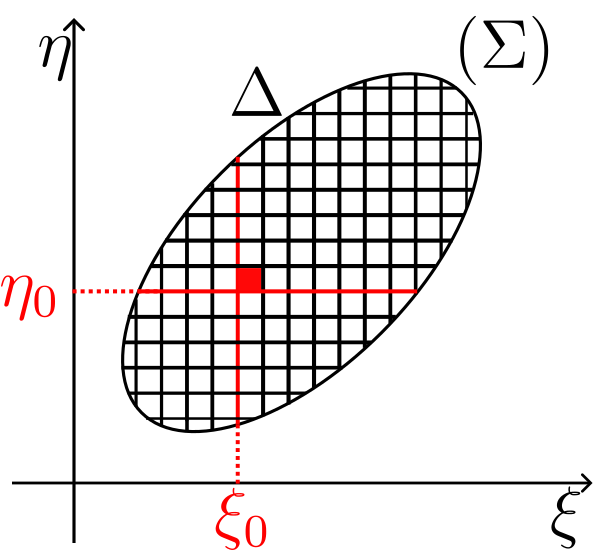
\includegraphics[scale=0.7]{8.16.2.png}
  \end{minipage}
  \vspace{1em}
  \par
  Пусть в области $\Delta$ задана системой непрерывных функций:
  $\begin{cases}
    x=x(\xi,\eta)\\
    y=y(\xi,\eta)
  \end{cases} (1)$\\
  Если различными (.) $(\xi;\eta) \in \Delta$ отвечают различные (.) $(x,y) \in D,$ то система (1)
  однозначно разрешима относительно $\xi$ и $\eta$.
  $\begin{cases}
    \xi=\xi(x;y)\\
    \eta=\eta(x;y)
  \end{cases} (2)$\\
  \underline{Определение: } $\frac{D(x;y)}{D(\xi,\eta)}=
  \begin{vmatrix}
    \frac{\delta x}{\delta \xi} & \frac{\delta x}{\delta \eta}\\
    \frac{\delta y}{\delta \xi} & \frac{\delta y}{\delta \eta}
  \end{vmatrix}$ Якобиан перехода из КСК в ДСК.\\
  \begin{itemize}
    \item Если $\frac{D(x;y)}{D(\xi;\eta)} \not = 0,$ то внутренней (.) $\xi,\eta$ соответствует
    внутренней (.) (x;y).\\Граничной (.) $(\xi,\eta)$ соответствует граничная (.) $(x;y)$
    \item Если $\frac{D(x;y)}{D(\xi;\eta)} > 0$, то при переходе в ДСК, направление обхода не меняется.
    \item Если $\frac{D(x;y)}{D(\xi;\eta)} < 0$, то при переходе в ДСК, направление обхода поменяется.
    \item Если в $\Delta$ взять гладкую кривую, то с помощью (1):
    $\begin{matrix}
        \begin{cases}
          \xi=\xi(t)\\
          \eta=\eta(t)
        \end{cases} \alpha\leq t\leq\beta\\
        \begin{cases}
          x=x(\xi(t);\eta(t))=x(t)\\
          y=y(\xi(t);\eta(t))=y(t)
        \end{cases} (3)
      \end{matrix}$
  \end{itemize}
  \underline{Примеры:}\\
  a)ПСК
  \[\begin{matrix}
    x=r\cos(\varphi) & r=\sqrt{x^2+y^2}\\
    y=r\sin(\varphi) & \varphi=
    \begin{cases}
      \arcctg \frac{y}{x},(.) (x;y) \in \text{ I, II ч.}\\
      \arcctg \frac{y}{x}+\pi,(.) (x;y) \in  \text{II,III ч.}\\
    \end{cases}
  \end{matrix}\]\\
  \break
  б) Семейство пересекающих парабол.
  \[y^2 =2px \hspace{20pt} x^2=2qy\] 
  \begin{minipage}{0.45\textwidth}
    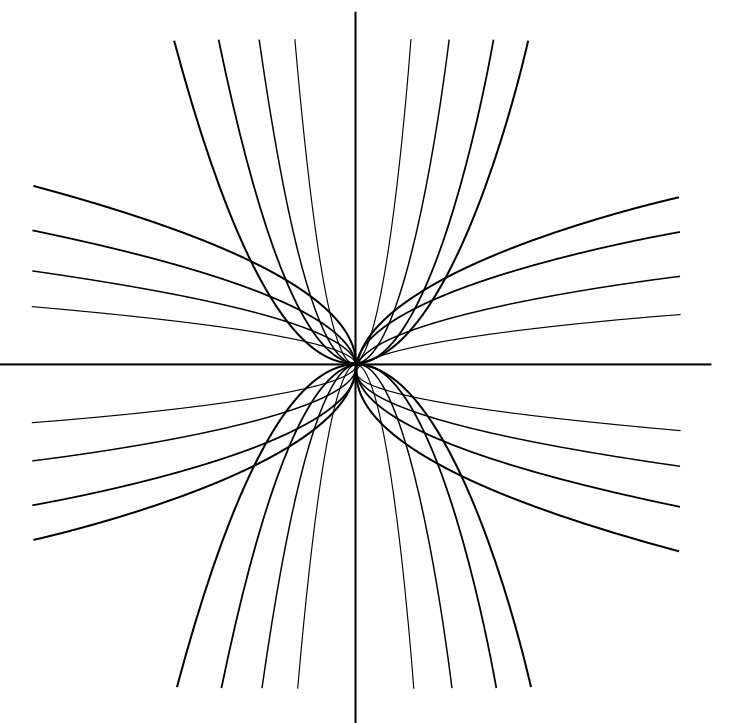
\includegraphics[scale=0.6]{8.16.3.png}
  \end{minipage}
  \hspace{1em}
  \begin{minipage}{0.55\textwidth}
    $\text{ Пусть } 2p=\xi \hspace{20pt} 2q=\eta$\\
    $y^2=\xi x \hspace{20pt} x^2=\eta y$\\
    $x^4=\eta^2y^2=\eta^2 \xi x$\\
    $x^3=\eta^2 \xi$\\
    $\begin{vmatrix}
      x=\sqrt[3]{\eta^2 \xi}\\
      y=\sqrt[3]{\xi^2 \eta}
    \end{vmatrix} 
    \begin{matrix}
      \xi=\frac{x}{y^2}\\
      \eta=\frac{y}{x^2}
    \end{matrix}$
  \end{minipage}
  \vspace{1em}
  \par
  \subsection*{II Вычисление площади в криволинейной системе координат:}
  Рассмотри область $D \in x;y,$ ограниченную кусочно-гладкую контуром L. Пусть существует (1) и (2).
  Пусть существует $\frac{\delta^2 y}{\delta \xi \delta \eta}$ и она непрерывна. Найти $S_D$.\\
  \[S_D =\int_{(L)}xdy=
  \begin{vmatrix}
    x=x(t)\\
    y=y(t)\\
    \alpha \leq t \leq \beta\\
    \text{\underline{Замечание:} при изменении t от } \alpha \text{ до } \beta\\
     \text{L - положительный контур.}
  \end{vmatrix} 
  = \int_{a}^{b} x(t)y'(t)dt \overset{(3)}{=} \] 
  \[\overset{(3)}{=} \int_{\alpha}^{\beta} x(\xi(t),\eta(t))
  \Big[ \frac{\delta y}{\delta \xi}\xi'(t)+\frac{\delta y}{\delta \eta}\eta'(t)\Big]dt \boxed{=}\]\\
  Рассмотрим $\int_{\Sigma} x(\xi;\eta) \Big[\frac{\delta y}{\delta\xi}d\xi + \frac{\delta y}{\delta \eta}d \eta\Big]
  \rightarrow \int_{\alpha}^{\beta}x(\xi(t);\eta(t))\Big[ \frac{\delta y}{\delta \xi} \xi'(t)+
  \frac{\delta y}{\delta \eta}\eta'(t)\Big]dt$\\
  \[\boxed{=} \pm \int_{\Sigma}x(\xi(t);\eta(t)) \Big[\frac{\delta y}{\delta\xi}d\xi + \frac{\delta y}{\delta \eta}d \eta\Big]
  \boxed{=}
  \begin{matrix}
    \text{"+", если положительный обход у L соответствует} \\
    \text{положительному обходу } \Sigma\\
    \text{"-", если положительный обход у L соответствует} \\
    \text{отрицательному обходу } \Sigma
  \end{matrix}\]
  \begin{center}
    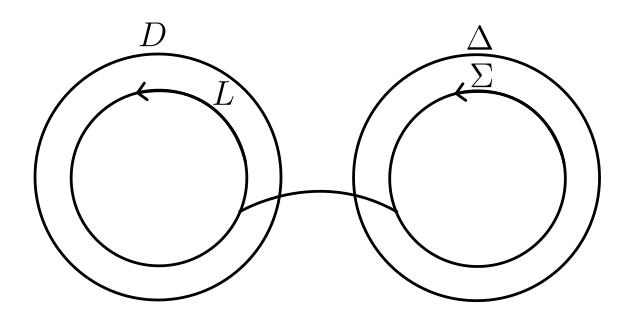
\includegraphics[scale=0.7]{8.16.4.png}
  \end{center}
  \subsection*{Формула Грина:}
  \[\int_{(L)} Pdx+Qdy=\iint_D \Big[ \frac{\delta Q}{\delta x} - \frac{\delta P}{\delta y}\Big] dxdy\]
  \[\int_{(\Sigma)}P(\xi;\eta)d\xi+Q(\xi;\eta)d\eta= \iint_{\Delta} \Big[\frac{\delta Q}{\delta \xi} -\frac{\delta P}{\delta \eta} d\xi d\eta \Big]\]
  \[P(\xi;\eta)=x \frac{\delta y}{\delta \xi} \hspace{20pt} Q(\xi;\eta)=x \frac{\delta y}{\delta \eta}\]
  \[\frac{\delta Q}{\delta \xi}=\frac{\delta}{\delta \xi}(x \frac{\delta y}{\delta \eta})=
  \frac{\delta x}{\delta \xi}\frac{\delta y}{\delta \eta}+x\frac{\delta^2y}{\delta\xi \delta\eta}\]
  \[\frac{\delta P}{\delta \eta}=\frac{\delta}{\delta \eta}(x \frac{\delta y}{\delta \xi})=
  \frac{\delta x}{\delta \eta} \frac{\delta y}{\delta \xi}+x \frac{\delta^2 y}{\delta \eta \delta \xi}\]
  \[\frac{\delta Q}{\delta \xi}-\frac{\delta P}{\delta \eta}=\frac{\delta x}{\delta \xi} \frac{\delta y}{\delta \eta}-
  \frac{\delta x}{\delta \eta}\frac{\delta y}{\delta \xi}=
  \begin{vmatrix}
    \frac{\delta x}{\delta \xi} & \frac{\delta x}{\delta \eta}\\
    \frac{\delta y}{\delta \xi} & \frac{\delta y}{\delta \eta}\\
  \end{vmatrix} = \frac{D(x;y)}{D(\xi;\eta)}\]\\
  \[\boxed{=} \pm \iint_\Delta \frac{D(x;y)}{D(\xi;\eta)}d\xi d\eta \overset{\text{опр Якобиана}}{=} 
  \underbracket{\iint_\Delta \Big|\frac{D(x;y)}{D(\xi;\eta)}\Big|d\xi d\eta \boxed{=}}\]
  Теорема Лагранжа:
  \[f(b)-f(a)=f'(\xi)(b-a) \hspace{20pt} 
  \begin{matrix}
    \varepsilon = f'(\xi)\delta\\
    \lim_{\lambda_R \to 0} \frac{\varepsilon}{\delta}=f'(\xi)
  \end{matrix} \hspace{20pt} f'(\xi)=\frac{\varepsilon}{\delta}\]
  $f'(\xi)$ является коэффициентом растяжение(сжатия) прямой x в прямоугольнике в данной её (.)($\xi$)\\
  \[\overset{\hyperref[th:8.12.1]{\text{Теорема о среднем}}}{\boxed{=}}
  \Big|\frac{D(x;y)}{D(\xi;\eta)} \Big|_{M \in \Delta} \hspace{20pt} S_\Delta=S_D\]
  \[\iint_D f(x;y)dxdy=f(\xi;\eta)\iint_D dxdy = f(\xi;\eta)S_D\]
  \[\Big| \frac{D(x;y)}{D(\xi;\eta)}\Big|_{M \in \Delta} = \lim_{\Delta \to M} \frac{S_D}{S_\Delta}\]
  Модуль величины Якобиана в (.) есть коэффициент растяжения (сжатия) плоскости $\xi \eta$ при преобразовании
  её в плоскость $xy$
  \subsection*{III Замена переменных в двойном интеграле:}
  Рассмотрим $\iint_{D} f(x;y)dxdy$\\
  \begin{enumerate}
    \item Разбиваем область D кусочно-гладкими кривыми
    \item Разбиение R и так далее
  \end{enumerate}
  \[\sigma_R = \sum_{i=0}^{n-1} f(x_i;y_i)S_{D_i} =\sum_{i=0}^{n-1} f(x_i;y_i) \Big| I \Big| \Big|_{\overline{M_i}(\xi_i;\eta_i)}
  * S_{\Delta_i} \boxed{=} \]
  \begin{center}
    Так как $(x_i;y_i)$ - произвольная (.), то выберем её так\\ 
    чтобы в области $D_i$ ей соответствовала (.) $(\overline{\xi_i};\overline{\eta_i})$ в $\Delta_i$
  \end{center}
  \[\boxed{=} \sum_{i=0}^{n-1} f(x(\overline{\xi_i},\overline{\eta_i});y(\overline{\xi_i},\overline{\eta_i}))
  |I|_{\overline{M_i}(\xi_i;\eta_i)}S_{\Delta_i}\]
  \[\lim_{\lambda_R \to 0} \sigma_R \iint_D f(x(\xi;\eta);y(\xi;\eta))|I|d\xi d\eta\]
  Для ПСК: 
  $
  \begin{matrix}
    x=r\cos\varphi\\
    y=r\sin\varphi
  \end{matrix} \hspace{20pt}
  I = \begin{vmatrix}
    \frac{\delta x}{\delta r} & \frac{\delta x}{\delta \varphi}\\
    \frac{\delta y}{\delta r} & \frac{\delta y}{\delta \varphi}
  \end{vmatrix}=
  \begin{vmatrix}
    \cos\varphi & -r\sin\varphi\\
    \sin \varphi & r\cos\varphi 
  \end{vmatrix} = r\cos^2\varphi+r\sin^2\varphi=r
  $
  \[|I|=r\]
  \subsection{Приложения двойных интегралов.}
  \begin{enumerate}
    \item \[S_D=\iint_D dxdy\]
    \item \[V=\iint_D f(x;y)dxdy=\iint_{\overline{D}} f(x;z)dxdz = \iint_{\overline{\overline{D}}}f(y;z) dydz
    =\iint_{\overline{\overline{\overline{D}}}}F(x(u;v);y(u;v);z(u;v))dudv\]
    \item \[m=\iint_D \underbrace{\rho}_{\frac{kg}{m^2}}dxdy\]
    \item \[
    \begin{matrix}
      M_x=\iint \rho y dxdy & M_y=\iint_{\rho}\rho xdxdy\\
      x_c=\frac{M_y}{m} & y_c=\frac{M_x}{m}
    \end{matrix}\]
  \end{enumerate}
  \subsection{Площадь поверхности.}
  Пусть $Z=f(x;y)$. Можно говорить о верхней и нижней стороне поверхности. Если поверхность замкнута,
  то можно говорить о внешней стороне поверхности и о внутренней. Возьмём на поверхности произвольную
  (.) $m_0$, проведем в ней нормаль. И проведем из (.) $m_0$ замкнутый контур, начиная и заканчивая 
  в (.) $m_0$(при этом нормаль изменяется непрерывно). При возврате в (.) $m_0$ можно получить 2 
  варианта: 
  \begin{enumerate}
    \item вектор нормали сохранил своё направление;
    \item вектор нормаль поменяет непрерывные на противоположные.
  \end{enumerate}
  \underline{Определение: } Если при обходе по контуру нормаль меняет направление на противоположное,
  то поверхность называется односторонней. Если не поменяет по замкнутому контуру - двусторонней.\\
  \begin{minipage}{0.54\textwidth}
    \underline{Пример:} лист Мёбиуса - односторонняя поверхность. 
  \end{minipage}
  \hspace{1em}
  \begin{minipage}{0.3\textwidth}
    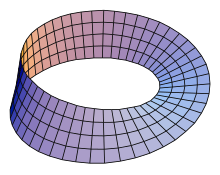
\includegraphics[scale=1]{8.18.1.png}
  \end{minipage}
  \vspace{1em}
  \par
  \underline{Определение: } Совокупность всех (.) поверхности с приписанными в них направлениями 
  нормалей называется стороной поверхности.\\
  \underline{Ориентация поверхностей}: 
  \begin{itemize}
    \item Верхняя сторона поверхности (острый угол с осью $OZ$) и замкнутую поверхность (внешняя сторона) 
    будем считать положительно ориентированными(правая ориентация)
    \item Нижняя сторона поверхности или внутренняя сторона(замкнутая поверхность) будем считать
    отрицательной ориентацией(левая ориентация)
  \end{itemize}
  \underline{Площадь поверхности}: Рассмотрим не замкнутую гладкую поверхность $S$, ограниченную
  кусочно-гладким контуром L.\\
  Разложим эту поверхность на элементарные $S_1,\dots,S_n$\\
  В каждой элементарной $S_i$ выберем произвольную (.) $M_i$ и в этой (.) проведем касательную
  плоскость к $S_i$\\
  \par
  \begin{minipage}{0.45\textwidth}
    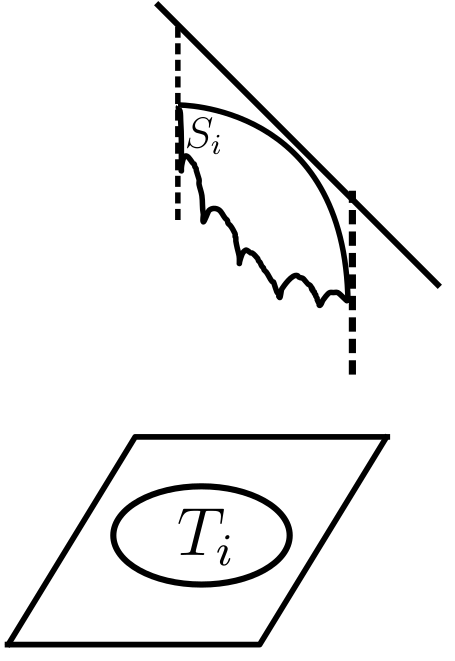
\includegraphics[scale=0.6]{8.18.2.png}
  \end{minipage}
  \hspace{1em}
  \begin{minipage}{0.55\textwidth}
    Построим на границе области $S_i$ цилиндрическую поверхность с образующими || оси OZ.Пересечение
    этого цилиндра с касательной плоскостью образует плоскую фигуру $T_i$.
    \[\text{Тогда }S=\lim_{\lambda_R \to 0} \Sigma \Delta T_i\]
  \end{minipage}
  \vspace{1em}
  \par
  Пусть поверхность задана:
  \[
  \begin{matrix}
    x=x(u;v)\\
    y=y(u;v)\\
    z=z(u;v)
  \end{matrix} \hspace{20pt}
  \begin{cases}
    x=r\cos(u)\\
    y=r\sin(u)\\
    z=v
  \end{cases} \text{ - цилиндрическая поверхность}
  \]
  Пусть $\mu' \in S \hspace{20pt} \mu'(x';y';z')$. Пересечем СК в (.) $\mu'$ и перейдем к новой
  СК $\xi \eta \chi$.\\
  \break
  \underline{Формулы преобразования координат:}
  \[\xi=(x-x')\cos(\alpha_1)+(y-y')\cos(\beta_1)+(z-z')\cos(\gamma_1)\]
  \[\eta=(x-x')\cos(\alpha_2)+(y-y')\cos(\beta_2)+(z-z')\cos(\gamma_2)\]
  \[\chi=(x-x')\cos(\alpha_3)+(y-y')\cos(\beta_3)+(z-z')\cos(\gamma_3)\]
  \begin{tabular}{ p{10pt}|p{10pt}|p{10pt}|p{10pt} }
    & X & Y & Z\\
    \hline
    $\xi$ & $\alpha_1$ & $\beta_1$ & $\gamma_1$\\
    \hline
    $\xi$ & $\alpha_2$ & $\beta_2$ & $\gamma_2$\\
    \hline
    $\xi$ & $\alpha$ & $\beta$ & $\gamma$\\
  \end{tabular}
  \hspace{20pt} $T_i = \iint_{D_{UV}}dudv=\iint_{D_{\xi \eta}}\Big| \frac{D(\xi;\eta)}{D(u;v)}\Big|
  d \xi d \eta$
  \[\frac{D(\xi;\eta)}{D(u;v)}=
  \begin{vmatrix}
    \frac{\delta \xi}{\delta u} &\frac{\delta \xi}{\delta V}\\
    \frac{\delta\eta}{\delta u} &\frac{\delta \eta}{\delta V}
  \end{vmatrix}=
  \]
  \[=\Big|
  \begin{matrix}
  \frac{\delta \xi}{\delta x}\frac{\delta x}{\delta u}+\frac{\delta \xi}{\delta y}\frac{\delta y}{\delta u}+
  \frac{\delta \xi}{\delta z}\frac{\delta Z}{\delta u} = x'_u\cos(\alpha_1)+y'_u\cos(\beta_1)+z'_u\cos(\gamma_1) & x'_u\cos(\alpha_1)+y'_u\cos(\beta_1)+z'_u\cos(\gamma_1) \\
  x'_v\cos(\alpha_2)+y'_v\cos(\beta_2)+z'_v\cos(\gamma_2) & x'_v\cos(\alpha_2)+y'_v\cos(\beta_2)+z'_v\cos(\gamma_2) 
  \end{matrix}\Big| =
  \]
  \[\begin{vmatrix}
    \begin{pmatrix}
      x'_u & y'_u & z'_u\\
      x'_v & y'_v & z'_v
    \end{pmatrix}
    \begin{pmatrix}
      \cos(\alpha_1)& \cos(\alpha_2)\\
      \cos(\beta_1)&\cos(\beta_2)\\
      \cos(\gamma_1)&\cos(\gamma_2)
    \end{pmatrix}
  \end{vmatrix}=\]
  \[=\underbrace{\begin{vmatrix}
    y'_u & z'_u\\
    y'_v & z'_v
  \end{vmatrix}}_{A}
  \underbrace{\begin{vmatrix}
    \cos(\beta_1) & \cos(\gamma_1)\\
    \cos(\beta_2) & \cos(\gamma_2)
  \end{vmatrix}}_{\cos(\alpha)}
  +
  \underbrace{\begin{vmatrix}
    z'_u&x'_u\\
    z'_v&x'_v
  \end{vmatrix}}_{B}
  \underbrace{\begin{vmatrix}
    \cos(\gamma_1) & \cos(\alpha_1)\\
    \cos(\gamma_2)&\cos(\alpha_2)
  \end{vmatrix}}_{\cos(\beta)}
  +
  \underbrace{\begin{vmatrix}
    x'_u & y'_u\\
    x'_v & y'_v
  \end{vmatrix}}_{C}
  \underbrace{\begin{vmatrix}
    \cos(\alpha_1)&\cos(\beta_1)\\
    \cos(\alpha_2)&\cos(\beta_2)
  \end{vmatrix}}_{\cos(\gamma)}
  \boxed{=}\]
  \par
  \underline{Замечание:} Каждый из координатных ортов ($\overline{\cos(\alpha_1);\cos(\beta_1);\cos(\gamma_1)}$),($\overline{\cos(\alpha_2);\cos(\beta_2);\cos(\gamma_2)}$)
  ,($\overline{\cos(\alpha);\cos(\beta);\cos(\gamma)}$) взаимно перпендикулярны.
  Поэтому:
  \[(\overline{\cos(\alpha);\cos(\beta);\cos(\gamma)}) = 
  \begin{vmatrix}
    i&j&k\\
    \cos(\alpha_1)&\cos(\beta_1)&\cos(\gamma_1)\\
    \cos(\alpha_2)&\cos(\beta_2)&\cos(\gamma_2)
  \end{vmatrix}=\]
  \[= \overline{i}
  \equalto{
    \begin{vmatrix}
    \cos(\beta_1)&\cos(\gamma_1)\\
    \cos(\beta_2)&\cos(\gamma_2)
    \end{vmatrix}
  }{\cos(\alpha)}+ \overline{j}
  \begin{vmatrix}
    \cos(\alpha_1)&\cos(\gamma_1)\\
    \cos(\alpha_2)&\cos(\gamma_2)
  \end{vmatrix}
  + \overline{k}
  \begin{vmatrix}
    \cos(\alpha_1)&\cos(\beta_1)\\
    \cos(\alpha_2)&\cos(\beta_2)
  \end{vmatrix}
  \]
  \[\boxed{=}A\cos(\alpha)+B\cos(\beta)+C\cos(\gamma)\boxed{=}\]
  \underline{Определение: } Если поверхность задана $\begin{matrix}
    x=x(u;v)\\
    y=y(u;v)\\
    z=z(u;v)
  \end{matrix}$, то нормаль к поверхности задается$\begin{vmatrix}
    \overline{i}&\overline{j}&\overline{k}\\
    x'_u & y'_u & z'_u\\
    x'_v & y'_v & z'_v
  \end{vmatrix}=(n_x;n_y;n_z)=\overline{(A;B;C)}$\\
  \underline{Пример:}\\
  \[\begin{matrix}
    \text{Рассмотрим } z=f(x;y)\\
    u=x\\
    v=y
  \end{matrix}
  \hspace{20pt}
  \begin{vmatrix}
    \overline{i}&\overline{j}&\overline{k}\\
    1&0&z'_x\\
    0&1&z'_y 
  \end{vmatrix}=
  \begin{matrix}
    \overline{i}(-z'_x)-jz'_y+\overline{k}\\
    (-z'_x;-z'_y;1) \text{ или }\\
    (z'_x;z'_y;-1)
  \end{matrix}\]
  \underline{С другой стороны:}
  \[
  \cos(\alpha)=\frac{A}{\pm \sqrt{A^2+B^2+C^2}}\\
  \cos(\beta)=\frac{B}{\pm \sqrt{A^2+B^2+C^2}}\\
  \cos(\gamma)=\frac{C}{\pm \sqrt{A^2+B^2+C^2}}
  \]
  Пусть $A',B',C'$ - значения определителей $A,B,C$ в (.) $\mu'$
  \[\boxed{=}
  \frac{AA'+BB'+CC'}{\pm \sqrt{A^2+B^2+C^2}}
  \boxed{=}\]
  Если расстояние между (.) ($u;v$) и ($u';v'$) стремится к нулю, то $\frac{D(\xi;\eta)}{D(u;v)} = \sqrt{A'^2+B'^2+C'^2}+\varepsilon'$
  \[
  S_{T_i}=\iint_{D_{uv}}\sqrt{A^2+B^2+C^2}dudv+\varepsilon;S_\text{поверхности}=\lim_{\lambda_R \to 0}\Sigma S_{T_i}=\iint_{D_{uv}}\sqrt{A^2+B^2+C^2}dudv=S
  \]
  \[
  \text{Рассмотрим }
  \begin{pmatrix}
    x_u & y'_u &z'_u\\
    x'_v&y'_v&z'_v
  \end{pmatrix}
  \begin{pmatrix}
    x'_u &x'_v\\
    y'_u&y'_v\\
    z'_u&z'_v
  \end{pmatrix}
  =
  \begin{pmatrix}
    x'^2_u+y'^2_u+z'^2_u & x'_u x'_v+y'_u y'_v+ z'_u z'_v\\
    \underbrace{x'_u x'_v+y'_u y'_v+ z'_u z'_v}_F & \underbrace{x'^2_v+y'^2_v+z'^2_v}_{G}
  \end{pmatrix}
  \]
  \[
  \text{Рассмотрим } \begin{vmatrix}
    E & F\\
    F & G
  \end{vmatrix} =EG-F^2=A^2+B^2+C^2 \hspace{20pt} S=\iint_{D_{uv}}\sqrt{EG-F^2}dudv
  \]
  $\text{Рассмотрим } Z=f(x;y) \text{ уравнение поверхности}.
  \begin{matrix}
    u \sim x\\
    v \sim y
  \end{matrix}$ 
  \[ A=
  \begin{vmatrix}
    y'_u & z'_u \\
    y'_v & z'_v
  \end{vmatrix} =\begin{vmatrix}
    0 & z'_x\\
    1 & z'_y
  \end{vmatrix}=-z'_x\]
  \[ B=
  \begin{vmatrix}
    z'_u & x'_u \\
    z'_v & x'_v
  \end{vmatrix} =\begin{vmatrix}
    z'_x & 1\\
    z'_y & 0
  \end{vmatrix}=-z'_y\]
  \[ C=
  \begin{vmatrix}
    x'_u & y'_x\\
    x'_v & y'_y
  \end{vmatrix} =\begin{vmatrix}
    1 & 0\\
    0 & 1
  \end{vmatrix}=1\]
  \[S=\iint_{D_{xy}}\sqrt{1 + z'^2_x + z'^2_y}dxdy\]
  Рассмотрим $\cos(\gamma)=\frac{C}{\pm \sqrt{A^2+B^2+C^2}}=\frac{1}{\pm \sqrt{1+z'^2_x+z'^2_y}}$
  \[S=\iint_{D_{xy}}\sqrt{1+z'^2_x+z'^2_y}dxdy=\iint_{D_{xy}}\frac{dxdy}{|\cos(\gamma)|} \hspace{20pt} \gamma - \forall \text{ угол}\]
  \break
  \subsection{Поверхностные интегралы I и II рода.}
  Пусть в каждой (.) двусторонней гладкой(или кусочно-гладкой) поверхности, ограниченной кусочно-гладким контуром
  определена функция f(x;y;z)
  \begin{enumerate}
    \item Производим разбиение R поверхности
    \item Выберем (.) $\mu_i$ произвольно: $\mu_i \in S_i$
    \item Вычислим $f(\mu_i) = f(x_i;y_i;z_i)$
    \item Вычислим $f(x_i;y_i;z_i)\Delta S_i$
    \item Составим $\sigma_R=\sum_{i=0}^{n-1}f(x_i;y_i;z_i)\Delta S_i$
    \item Вычислим $\lim_{\lambda_R \to 0} \sigma_R = \iint_{S} f(x;y;z)dS$
  \end{enumerate}
  \underline{Определение: }Если существует конечный $\lim_{\lambda_R \to 0}$, не зависящий от способа разбиения поверхности
  S и выбора (.) $\mu_i$ , то он называется поверхностным интегралом I рода от функции $f(x;y;z)$ по поверхности S.\\
  \underline{Вычисление: } 
  \[ \iint_S f(x;y;z)dS=\iint_{D_{xy}}f(x;y;z(x;y)) \sqrt{1+z'^2_x+z'^2_y}dxdy = 
  \iint_{D_{uv}} f(x(u;v);y(u;v);z(u;v))\sqrt{EG-F^2}dudv\]
  \subsection*{Поверхностные интегралы II рода:}
  Пусть в каждой (.) двусторонней гладкой(или кусочно-гладкой) поверхности, ограниченной кусочно-гладким контуром
  определена функция $f(x;y;z)$.\\ Выберем одну из сторон поверхности:
  \begin{enumerate}
    \item Произведем разбиение R к поверхности
    \item Выберем (.) $\mu_i$ произвольно: $\mu_i \in S_i$
    \item Вычислим $f(\mu_i)=f(x;y;z)$
    \item Вычислим $f(x_i;y_i;z_i)\Delta D_i; \hspace{20pt} \Delta D_i$ - проекция $S_i$ на плоскость $Dy$\\
    Проекция берется со знаком "+", если вектор нормали к поверхности образует острый угол с осью $OZ$. "-" если угол
    между нормалью и $OZ$ тупой.
    \item Составим $\sigma_R=\sum_{i=0}^{n-1}f(x_i;y_i;z_i)\Delta D_i$
    \item $\lim_{\lambda_R \to 0}\sigma_R=\iint_S f(x;y;z)dxdy$
  \end{enumerate}
  \underline{Определение: }  Если существует конечный $\lim_{\lambda_R \to 0}$, не зависящий от способа разбиения
  поверхности S и выбора (.) $\mu_i$, то он называется поверхностным интегралом II рода от функции $f(x;y;z)$ по 
  поверхности S.\\
   \[\text{Аналогично: }\iint_S f(x;y;z)dxdz, \iint_S f(x;y;z)dydz\]
  \[\iint_S P(x;y;z)dydz+Q(x;y;z)dxdz+R(x;y;z)dxdy\text{ - поверхностный интеграл II рода общего вида}\]
  \underline{Вычисление: }
  \[\iint_S f(x;y;z)dxdy = \pm \iint_{D_{xy}} f(x;y;z(x;y))dxdy\]
  \subsection{Связь между поверхностными интегралами}
\end{document}